% Options for packages loaded elsewhere
\PassOptionsToPackage{unicode}{hyperref}
\PassOptionsToPackage{hyphens}{url}
\PassOptionsToPackage{dvipsnames,svgnames,x11names}{xcolor}
%
\documentclass[
  12pt,
]{article}
\usepackage{amsmath,amssymb}
\usepackage{lmodern}
\usepackage{setspace}
\usepackage{iftex}
\ifPDFTeX
  \usepackage[T1]{fontenc}
  \usepackage[utf8]{inputenc}
  \usepackage{textcomp} % provide euro and other symbols
\else % if luatex or xetex
  \usepackage{unicode-math}
  \defaultfontfeatures{Scale=MatchLowercase}
  \defaultfontfeatures[\rmfamily]{Ligatures=TeX,Scale=1}
\fi
% Use upquote if available, for straight quotes in verbatim environments
\IfFileExists{upquote.sty}{\usepackage{upquote}}{}
\IfFileExists{microtype.sty}{% use microtype if available
  \usepackage[]{microtype}
  \UseMicrotypeSet[protrusion]{basicmath} % disable protrusion for tt fonts
}{}
\makeatletter
\@ifundefined{KOMAClassName}{% if non-KOMA class
  \IfFileExists{parskip.sty}{%
    \usepackage{parskip}
  }{% else
    \setlength{\parindent}{0pt}
    \setlength{\parskip}{6pt plus 2pt minus 1pt}}
}{% if KOMA class
  \KOMAoptions{parskip=half}}
\makeatother
\usepackage{xcolor}
\usepackage[left=4cm, right=3cm, top=2.5cm, bottom=2.5cm]{geometry}
\usepackage{longtable,booktabs,array}
\usepackage{calc} % for calculating minipage widths
% Correct order of tables after \paragraph or \subparagraph
\usepackage{etoolbox}
\makeatletter
\patchcmd\longtable{\par}{\if@noskipsec\mbox{}\fi\par}{}{}
\makeatother
% Allow footnotes in longtable head/foot
\IfFileExists{footnotehyper.sty}{\usepackage{footnotehyper}}{\usepackage{footnote}}
\makesavenoteenv{longtable}
\usepackage{graphicx}
\makeatletter
\def\maxwidth{\ifdim\Gin@nat@width>\linewidth\linewidth\else\Gin@nat@width\fi}
\def\maxheight{\ifdim\Gin@nat@height>\textheight\textheight\else\Gin@nat@height\fi}
\makeatother
% Scale images if necessary, so that they will not overflow the page
% margins by default, and it is still possible to overwrite the defaults
% using explicit options in \includegraphics[width, height, ...]{}
\setkeys{Gin}{width=\maxwidth,height=\maxheight,keepaspectratio}
% Set default figure placement to htbp
\makeatletter
\def\fps@figure{htbp}
\makeatother
\setlength{\emergencystretch}{3em} % prevent overfull lines
\providecommand{\tightlist}{%
  \setlength{\itemsep}{0pt}\setlength{\parskip}{0pt}}
\setcounter{secnumdepth}{5}
\usepackage[utf8]{inputenc}
\usepackage[spanish,es-tabla]{babel}
\usepackage[fixlanguage]{babelbib}
\usepackage{geometry}
\geometry{letterpaper,left=2cm,top=2cm, right=2cm}
\usepackage{times}           
\usepackage{caption}
\captionsetup[figure, table]{labelfont={bf},labelformat={default},labelsep=period}
\usepackage{graphicx}
\usepackage{booktabs}
\usepackage{longtable}
\usepackage{array}
\usepackage{multirow}
\usepackage{wrapfig}
%\usepackage{float}
\usepackage{colortbl}
\usepackage{xcolor}
\usepackage{pdflscape}
\usepackage{tabu}
\usepackage{threeparttable}
\usepackage{pdfpages}
\usepackage{hyphsubst}
\usepackage{floatrow}
\usepackage{float}
\floatsetup[figure]{capposition=top}
\floatsetup[table]{capposition=top}
\usepackage{booktabs}
\usepackage{longtable}
\usepackage{array}
\usepackage{multirow}
\usepackage{wrapfig}
\usepackage{float}
\usepackage{colortbl}
\usepackage{pdflscape}
\usepackage{tabu}
\usepackage{threeparttable}
\usepackage{threeparttablex}
\usepackage[normalem]{ulem}
\usepackage{makecell}
\usepackage{xcolor}
\ifLuaTeX
  \usepackage{selnolig}  % disable illegal ligatures
\fi
\IfFileExists{bookmark.sty}{\usepackage{bookmark}}{\usepackage{hyperref}}
\IfFileExists{xurl.sty}{\usepackage{xurl}}{} % add URL line breaks if available
\urlstyle{same} % disable monospaced font for URLs
\hypersetup{
  pdftitle={Manual Metodológico ELSOC 2016-2022},
  pdfauthor={Equipo ELSOC},
  colorlinks=true,
  linkcolor={blue},
  filecolor={Maroon},
  citecolor={Blue},
  urlcolor={Blue},
  pdfcreator={LaTeX via pandoc}}

\title{Manual Metodológico ELSOC 2016-2022}
\author{Equipo ELSOC}
\date{}

\begin{document}
\maketitle

{
\hypersetup{linkcolor=}
\setcounter{tocdepth}{1}
\tableofcontents
}
\listoffigures
\listoftables
\setstretch{1.5}
\hypertarget{presentaciuxf3n}{%
\section*{Presentación}\label{presentaciuxf3n}}
\addcontentsline{toc}{section}{Presentación}

El Estudio Longitudinal Social de Chile (ELSOC) es una encuesta desarrollada para analizar intertemporalmente la evolución del conflicto y cohesión en la sociedad chilena, basándose en modelos conceptuales descritos en la literatura nacional e internacional que abordan dichas materias. Se orienta a examinar los principales antecedentes, factores moderadores y mediadores, así como las principales consecuencias asociadas al desarrollo de distintas formas de conflicto y cohesión social en Chile. Su objetivo fundamental es constituirse en un insumo empírico para la comprensión de las creencias, actitudes y percepciones de los chilenos hacia las distintas dimensiones de la convivencia y el conflicto, y como éstas cambian a lo largo del tiempo.

Esta encuesta fue diseñada por investigadores pertenecientes al Centro de Estudios de Conflicto y Cohesión Social (COES). COES está patrocinado por la Universidad de Chile y la Pontificia Universidad Católica de Chile, y cuenta con la Universidad Diego Portales y la Universidad Adolfo Ibáñez como instituciones asociadas. Si desea obtener más información sobre COES, visite la página web de COES (\url{www.coes.cl/}). COES es una iniciativa que desde 2013 cuenta con el financiamiento del \href{https://www.conicyt.cl/fondap/centros-fondap/}{Fondo de Financiamiento de Centros de Investigación en Áreas Prioritarias (FONDAP)} de la \href{https://www.conicyt.cl/}{Comisión Nacional de Investigación Científica y Tecnológica (CONICYT)}\footnote{\href{https://www.conicyt.cl/fondap/centros-fondap/centros-en-ejecucion/coes/}{Proyecto CONICYT/FONDAP/15130009}}, organismo dependiente del Ministerio de Educación de Chile. El levantamiento de datos de ELSOC se licita públicamente cada 2 años, y ha sido adjudicado en todas sus mediciones al \href{https://www.microdatos.cl/}{Centro MicroDatos de la Universidad de Chile (CMD)}.

El Manual se estructura en torno a secciones temáticas: la primera sección describe el diseño muestral del estudio panel, dividido en sus muestras original y refresco, y las actualizaciones que se han aplicado en el tiempo. La segunda sección describe el proceso de diseño del instrumento, lo cual es complementado con la ficha técnica del estudio. En el siguiente apartado se resumen los principales aspectos del trabajo de campo, enfatizando las particularidades del proceso de reentrevista a los participantes. El cuarto apartado corresponde al registro de versiones de la base de datos y detalla el protocolo de uso de éstas. Por último, se incluye un apartado con orientaciones básicas para el análisis y el libro de códigos de las variables incluidas en la base de datos.

\newpage

\hypertarget{dis_muest}{%
\section{Diseño Muestral del Estudio}\label{dis_muest}}

En el siguiente apartado se presenta la descripción del diseño muestral de ELSOC, correspondiente a la muestra original y a la muestra refresco del estudio. Al final de la sección se describen la construcción de los ponderadores de ELSOC.

\hypertarget{dis_muest_original}{%
\subsection{Diseño muestral Muestra original}\label{dis_muest_original}}

El diseño de la muestra original de ELSOC tuvo como objetivo conciliar los múltiples intereses de investigación de los investigadores asociados al Centro. Entre las consideraciones más relevantes destacaron las siguientes:

\begin{enumerate}
\def\labelenumi{\arabic{enumi}.}
\item
  Un diseño muestral que permitiera combinar las variables medidas en el cuestionario con las variables espaciales, registradas a nivel de manzana y comuna, contenidas en las bases de datos desarrolladas por el Centro de Inteligencia Territorial (CIT) de la Universidad Aldolfo Ibáñez. Dado que los datos del CIT no están disponibles para todas las manzanas del país, particularmente aquellas ubicadas en localidades rurales, se decidió incorporar en la muestra únicamente zonas urbanas. Esta consideración también coincidió con las preferencias de muchos investigadores del Centro, quiénes manifestaron estar principalmente interesados en una muestra de carácter urbano.
\item
  Algunos investigadores solicitaron un diseño que permitiera estimar modelos multi-nivel (o jerárquicos) agrupados por ciudad y comuna, y por tanto, se estabció que la muestra contuviera un número suficiente de ciudades y comunas, así como un número suficiente de casos dentro de cada cuidad y comuna, que permitiera tal análisis (Snijders \& Bosker, Capítulo 10).
\item
  Otros investigadores estaban interesados en comparar a los habitantes de las tres ciudades más grandes del país, lo que se tradujo en un diseño no proporcional que incrementara el número de encuestados en las zonas del Gran Valparaíso (ciudades de Viña del Mar y Valparaíso) y Gran Concepción (Concepción, Talcahuano y otras).
\item
  Finalmente, algunos investigadores solicitaron un diseño que permitiera comparar a los encuestados que vivieran en ciudades grandes y pequeñas, lo que favoreció incrementar el tamaño de la muestra de viviendas en ciudades pequeñas (Kish, 1965, Sección 3.5), particularmente aquellas con entre 30 mil y 100 mil habitantes.
\end{enumerate}

Los investigadores de COES trabajaron con la encargada del diseño muestral, Stephanie Eckman, para desarrollar un diseño que pudiera, razonablemente, cumplir con estas necesidades e intereses sustantivos. El diseño muestral final de la ola 1 de ELSOC COES proporciona una cobertura adecuada de las ciudades más grandes del país (Gran Santiago, Gran Valparaíso y Gran Concepción), así como ciudades más pequeñas, y también asegura la representación de personas en el norte y sur del país. En términos globales, el diseño muestral alcanza una representatividad aproximada del 77\% de la población total del país, y del 93\% de la población urbana. Las siguientes subsecciones detallan los distintos pasos del diseño de la muestra.

\hypertarget{preparaciuxf3n-del-marco-muestral}{%
\subsubsection*{Preparación del Marco Muestral}\label{preparaciuxf3n-del-marco-muestral}}
\addcontentsline{toc}{subsubsection}{Preparación del Marco Muestral}

El proceso de muestreo de la muestra original se realizó en base a los datos del pre-censo del año 2011, los cuales fueron formateados por el CIT. Aunque los recuentos de población del censo de 2012 no son precisos, el trabajo del pre-censo recolectando información sobre los viviendas en todos las manzanas (bloques) es de calidad. El conjunto de datos contenía un total de 155.757 bloques, pero se eliminaron cuatro tipos diferentes antes de que comenzara con la selección.

\begin{enumerate}
\def\labelenumi{\arabic{enumi}.}
\item
  Siguiendo los intereses analíticos de los investigadores del Centro, sólo se utilizaron bloques urbanos. Para determinar qué bloques eran urbanos, se empleó la codificación del tipo de localidad (urbana o rural) contenida en la base de datos del pre-censo de 2011. Consecuentemente, 22.188 (14,2\%) bloques fueron excluidos en este paso.
\item
  Nuevamente, en función de los intereses analíticos de los investigadores del Centro, sólo los bloques que habían sido previamente geo-referenciados por el CIT se conservaron para el muestreo. Esto implica que un total de 1.971 (1,5\% de los bloques urbanos) que no estaban geo-referenciados fueron removidos en este paso.
\item
  Sólo los bloques que contenían cinco o más viviendas (de acuerdo con el pre-censo de 2011) fueron retenidos. 503 bloques (menos del 1\% de los bloques restantes tras los pasos 1 y 2) no alcanzaron este umbral y fueron eliminados.
\item
  Sólo los bloques en las ciudades con más de 10.000 personas eran elegibles para la selección. 10.238 bloques (7.8\% de los bloques restantes) fueron excluidos del marco muestral.
\end{enumerate}

De esta forma, el marco muestral final contiene 120.857 bloques. La muestra de COES representará solamente estos bloques y no aquellos que fueron excluidos. Las estimaciones derivadas de los datos de la muestra se aplicarán únicamente a esta población objetivo y no deben aplicarse a toda la población chilena. El proceso de selección de entrevistados se desarrolló en cuatro etapas, aunque durante el trabajo de campo se añadió una quinta etapa.

\hypertarget{etapa1m1}{%
\subsubsection*{Etapa 1: Selección de Ciudades}\label{etapa1m1}}
\addcontentsline{toc}{subsubsection}{Etapa 1: Selección de Ciudades}

El universo de bloques (los 120.857 bloques mencionados) fue agregado al nivel de la ciudad, resultando en 122 ciudades. Las tres ciudades más grandes (Gran Santiago, Viña del Mar - Valparaiso y Concepción - Talcahuano) fueron seleccionadas con certeza. Las ciudades restantes son estratificadas por la población. La tabla \ref{tab:tabla-estratos} muestra las definiciones de los estratos y los tamaños de población y de muestra en cada uno.

\begin{table}[H]

\caption{\label{tab:tabla-estratos}Población por ciudad y tamaños de muestra, por estrato}
\centering
\resizebox{\linewidth}{!}{
\begin{tabular}[t]{l>{\centering\arraybackslash}p{4em}>{\centering\arraybackslash}p{4em}>{\centering\arraybackslash}p{4em}>{\centering\arraybackslash}p{4em}>{\centering\arraybackslash}p{4em}>{\centering\arraybackslash}p{4em}>{\centering\arraybackslash}p{4em}}
\toprule
\multicolumn{1}{c}{ } & \multicolumn{3}{c}{ } & \multicolumn{2}{c}{Estrato Norte} & \multicolumn{2}{c}{Estrato Sur} \\
\cmidrule(l{3pt}r{3pt}){5-6} \cmidrule(l{3pt}r{3pt}){7-8}
Estrato & Definición (N° habitantes) & Tamaño población ciudades & Tamaño muestra ciudades & Tamaño población estrato & Tamaño muestra estrato & Tamaño población estrato & Tamaño muestra estrato\\
\midrule
Gran Santiago &  & 1 & 1 &  &  &  & \\
Gran Valparaíso &  & 1 & 1 &  &  &  & \\
Gran Concepción &  & 1 & 1 &  &  &  & \\
Ciudades grandes & > 100 mil & 18 & 8 & 8 & 4 & 10 & 3\\
Ciudades medianas & > 30 mil & 28 & 10 & 15 & 6 & 13 & 3\\
\addlinespace
Ciudades pequeñas & > 10 mil & 73 & 19 & 24 & 6 & 49 & 13\\
\bottomrule
\end{tabular}}
\end{table}

Los estratos de ciudades grandes, ciudades medianas y ciudades pequeñas fueron estratificados geográficamente por zona Norte o Sur, para asegurar que la muestra contuviera ciudades del norte y sur de Chile. Esto redunda en un total de nueve estratos. La muestra se asignó entre las dos áreas en proporción al tamaño de su población en el universo. Véase la Tabla \ref{tab:tabla-estratos} para ver el detalle acerca de los tamaños de población y muestra en cada uno de los estratos norte y sur.

La selección de ciudades dentro de cada uno de estos estratos finales se realizó en forma proporcional al tamaño de la población de cada ciudad. Este método da mayores probabilidades de selección a las grandes ciudades.

La probabilidad de selección de una ciudad \(i\) dentro del estrato \(h\) fue:

\[\pi_i=\frac{(nc_h)(pop_i)}{\sum_h pop}\]

donde \(nc_h\) es el número de ciudades seleccionadas en el estrato \(h\) y \(pop_i\) es la población de ciudad \(i\).

\hypertarget{etapa2m1}{%
\subsubsection*{Etapa 2: Selección de Bloques (Manzanas)}\label{etapa2m1}}
\addcontentsline{toc}{subsubsection}{Etapa 2: Selección de Bloques (Manzanas)}

Las 40 ciudades seleccionadas contenían 87.839 bloques. En la segunda etapa se seleccionaron bloques en cada ciudad con población proporcional al tamaño, donde el tamaño fue determinado a partir del recuento de unidades de vivienda del pre-censo. La selección fue sistemática: la lista de bloques en las ciudades seleccionadas se ordenó según sub-distrito censal y número de bloque para asegurar que los bloques seleccionados se extendieran por toda la ciudad\footnote{Los números de bloques y distritos censales fueron entregados por Matías Garretón, investigador de CIT. Los sub-distritos censales son unidades geográficas más pequeñas que la comuna, pero más grandes que los bloques.}.

la Tabla \ref{tab:tabla-ciudades} muestra el número de bloques seleccionados en cada ciudad, según estrato. La muestra de bloques se asignó de manera desproporcionada para que las áreas fuera de Santiago estuvieran sobre-representadas en relación con su tamaño en la población objetivo. Varios investigadores COES solicitaron esta asignación para asegurar que la muestra fuera diversa con respecto al tamaño de la ciudad.

La probabilidad de selección de un bloque \(j\) en la ciudad \(i\), condicionada a la selección de la ciudad, fue:

\[\pi_{j|i}=\frac{(nb_i)(hu_j)}{\sum_i hu}\]

donde \(nb_i\) es el número de bloques seleccionadas en la ciudad \(i\) y \(hu_j\) es la población de la ciudad \(i\).

\begin{table}[H]

\caption{\label{tab:tabla-ciudades}Distribución de ciudades y bloques por estrato}
\centering
\begin{tabular}[t]{l>{\centering\arraybackslash}p{6em}>{\centering\arraybackslash}p{6em}>{\centering\arraybackslash}p{6em}c}
\toprule
Estrato & Definición (N° habitantes) & Tamaño muestra ciudades & Número de bloques por ciudad & Número de bloques\\
\midrule
Gran Santiago &  & 1 & 200 & 200\\
Gran Valparaíso &  & 1 & 100 & 100\\
Gran Concepción &  & 1 & 100 & 100\\
Ciudades grandes & > 100 mil & 8 & 26 & 208\\
Ciudades medianas & > 30 mil & 10 & 25 & 250\\
\addlinespace
Ciudades pequeñas & > 10 mil & 19 & 11 & 209\\
Total &  & 40 & 27 & 1080\\
\bottomrule
\end{tabular}
\end{table}

En 4 ciudades algunos bloques eran tan grandes que fueron selecciones certeras. Es decir, los recuentos de unidades de vivienda eran mayores que el intervalo de selección y se seleccionarían en cualquier muestra, e incluso podrían seleccionarse dos veces. Para evitar selecciones duplicadas, estos bloques se eligieron primero con certeza y luego se seleccionaron bloques adicionales entre los restantes para aquellas ciudades, de modo de alcanzar el tamaño de muestra total deseado para la ciudad (ver Tabla \ref{tab:tabla-ciudades}. \(\pi_{j|i}\) para estas ciudades es 1.

Los 1.067 bloques seleccionados en las 40 ciudades elegidas fueron enpadronados en terreno, con la finalidad de realizar la selección de los viviendas con la información más actualizada posible. El CIT proporcionó mapas de cada bloque seleccionado. El personal de campo de CMD visitó presencialmente cada bloque, y creó un empadronamiento de todas las unidades de vivienda de dichos bloques. Los listados fueron revisados cuidadosamente para detectar cualquier error o duplicado.

Durante el proceso de empadronamiento, el Centro de Microdatos encontró que algunos bloques tenían más de 100 viviendas, lo que dificulta excesivamente el proceso de empadronamiento. Consecuentemente, se dividieron estos bloques en sub-bloques de tamaño aproximadamente igual (40 a 50 viviendas) y seleccionaron uno para ser empadronado. Debido a que los sub-bloques fueron creados para ser de tamaños similares, estos fueron seleccionados en base a igual probabilidad. En total, 301 bloques fueron sub-muestreados. Los bloques restantes no se vieron afectados por esta etapa.

\hypertarget{etapa3m1}{%
\subsubsection*{Etapa 3: Selección de viviendas}\label{etapa3m1}}
\addcontentsline{toc}{subsubsection}{Etapa 3: Selección de viviendas}

El número de viviendas seleccionadas en cada bloque varió según el estrato, como se muestra en la Tabla \ref{tab:bloques}. Este diseño resultó en 4.001 unidades de vivienda, con lo cual se buscaba obtener aproximadamente 3.000 entrevistas completas, bajo el supuesto de una tasa de respuesta del 75\% para todos los estratos.

\begin{table}[H]

\caption{\label{tab:bloques}Distribución de viviendas por bloques, según estrato}
\centering
\begin{tabular}[t]{lcc}
\toprule
Estrato & Definición (N° habitantes) & Número de viviendas por bloque\\
\midrule
Gran Santiago &  & 5\\
Gran Valparaíso &  & 5\\
Gran Concepción &  & 5\\
Ciudades grandes & > 100 mil & 3\\
Ciudades medianas & > 30 mil & 3\\
\addlinespace
Ciudades pequeñas & > 10 mil & 3\\
Total &  & 4001\\
\bottomrule
\end{tabular}
\end{table}

Se realizó una muestra aleatoria simple de viviendas en cada bloque. La combinación de la población proporcional al tamaño de muestreo en las dos primeras etapas y el muestreo aleatorio simple en la tercera y cuarta etapas dio lugar a una muestra de viviendas con aproximadamente igual probabilidad dentro de cada uno de los nueve estratos.

La probabilidad de selección de un vivienda \(k\) en el bloque \(j\) en la ciudad \(i\) y el estrato \(h\) fue:

\[\pi_{k|j,i}=\frac{nh_j}{NH_j}\]

donde \(nh_j\) es el número de viviendas seleccionadas en el bloque \(j\), y \(NH_j\) corresponde al número de viviendas alistadas en el bloque \(j\).

\hypertarget{etapa4m1}{%
\subsubsection*{Etapa 4: Selección de personas}\label{etapa4m1}}
\addcontentsline{toc}{subsubsection}{Etapa 4: Selección de personas}

Los encuestadores visitaron cada vivienda seleccionado e intentaron llevar a cabo la entrevista. El primer paso en el proceso de la entrevista fue identificar al entrevistado objetivo. Cuando había más de un adulto en el vivienda, uno fue seleccionado usando una muestra aleatoria simple, usando una tabla de Kish.

La probabilidad de selección de una persona en el vivienda \(k\) fue:

\[\pi_{l|k,j,i}=\frac{1}{NP_j}\]

donde \(NP_j\) es el número de adultos (mayores a 18 años y menores de 75 años) que habitan la vivienda \(j\).

\hypertarget{etapa5m1}{%
\subsubsection*{Etapa 5: Aumento del tamaño muestral}\label{etapa5m1}}
\addcontentsline{toc}{subsubsection}{Etapa 5: Aumento del tamaño muestral}

Durante el trabajo de campo de la primera ola (2016), se observó que el supuesto de una tasa de respuesta del 75\% para todos los estratos era incorrecto. En primer lugar, la tasa de respuesta general fue inferior a 75\% y, en segundo lugar, hubo una significativa heteregoneidad en las tasas de respuestas entre regiones. Debido a esto, se decidió aumentar el número de viviendas por bloque para lograr efectivamente las 3.000 entrevistas.

Este aumento en el número de viviendas por bloque tiene un efecto limitado sobre la probabilidad de selección de cada vivienda. Solo afecta a la probabilidad calculada en la Etapa 3, ya que el número de viviendas disponibles es menor, pero no hay cambios en las probabilidades calculadas en las Etapas 1 y 2. Esto ocurre porque los bloques seleccionados (en la Etapa 2) fueron usados, y no se introdujeron nuevos bloques.

Durante este proceso se añadieron a la muestra del estudio un total de 1.082 nuevos viviendas, ubicados dentro de los bloques seleccionados. La asignación de estos nuevos viviendas no fue uniforme en todos los bloques del país. En cambio, se concentraron en cuatro regiones: Regiones de Coquimbo, O´Higgins, Metropolitana, y Biobío, donde los encuestadores tuvieron mayores problemas para contactar a los encuestados. La Tabla \ref{tab:tabla-aumento} detalla las comunas en que se aumentó el número de viviendas con respecto al diseño inicial, junto con el número total de viviendas incorporados por bloque.

\begin{longtable}[t]{llcc}
\caption{\label{tab:tabla-aumento}Número de viviendas agregados a la muestra según región y comuna}\\
\toprule
Región & Comuna & Total viviendas agregadas & Viviendas agregadas por bloque\\
\midrule
\endfirsthead
\caption[]{\label{tab:tabla-aumento}Número de viviendas agregados a la muestra según región y comuna \textit{(continued)}}\\
\toprule
Región & Comuna & Total viviendas agregadas & Viviendas agregadas por bloque\\
\midrule
\endhead

\endfoot
\bottomrule
\endlastfoot
\addlinespace[0.3em]
\multicolumn{4}{l}{\textbf{Coquimbo}}\\
\hspace{1em} & Coquimbo & 24 & 2\\
\hspace{1em} & La Serena & 28 & 2\\
\hspace{1em} & Salamanca & 22 & 2\\
\addlinespace[0.3em]
\multicolumn{4}{l}{\textbf{O’Higgins}}\\
\hspace{1em} & Doñihue & 10 & 1\\
\hspace{1em} & Rancagua & 42 & 2\\
\hspace{1em} & Santa Cruz & 11 & 1\\
\addlinespace[0.3em]
\multicolumn{4}{l}{\textbf{Biobío}}\\
\hspace{1em} & Chiguayante & 24 & 3\\
\hspace{1em} & Concepción & 75 & 3\\
\hspace{1em} & Coronel & 11 & 1\\
\hspace{1em} & Penco & 4 & 1\\
\hspace{1em} & Quillón & 6 & 1\\
\hspace{1em} & San Pedro de la Paz & 28 & 2\\
\addlinespace[0.3em]
\multicolumn{4}{l}{\textbf{Metropolitana}}\\
\hspace{1em} & Cerrillos & 9 & 3\\
\hspace{1em} & Colina & 12 & 3\\
\hspace{1em} & Curacaví & 14 & 2\\
\hspace{1em} & El Bosque & 8 & 2\\
\hspace{1em} & Estación Central & 12 & 3\\
\hspace{1em} & Huechuraba & 6 & 2\\
\hspace{1em} & Independencia & 6 & 2\\
\hspace{1em} & Isla de Maipo & 39 & 3\\
\hspace{1em} & La Cisterna & 9 & 3\\
\hspace{1em} & La Florida & 24 & 2\\
\hspace{1em} & La Granja & 6 & 2\\
\hspace{1em} & La Pintana & 12 & 2\\
\hspace{1em} & La Reina & 9 & 3\\
\hspace{1em} & Las Condes & 33 & 3\\
\hspace{1em} & Lo Barnechea & 9 & 3\\
\hspace{1em} & Lo Espejo & 6 & 2\\
\hspace{1em} & Lo Prado & 6 & 2\\
\hspace{1em} & Macul & 8 & 2\\
\hspace{1em} & Maipú & 32 & 2\\
\hspace{1em} & Ñuñoa & 16 & 2\\
\hspace{1em} & Padre Hurtado & 6 & 3\\
\hspace{1em} & Pedro Aguirre Cerda & 6 & 2\\
\hspace{1em} & Peñaflor & 30 & 2\\
\hspace{1em} & Peñalolén & 14 & 2\\
\hspace{1em} & Providencia & 7 & 3\\
\hspace{1em} & Pudahuel & 14 & 2\\
\hspace{1em} & Puente Alto & 32 & 2\\
\hspace{1em} & Quilicura & 12 & 2\\
\hspace{1em} & San Bernardo & 16 & 2\\
\hspace{1em} & San Joaquín & 6 & 2\\
\hspace{1em} & San Miguel & 9 & 3\\
\hspace{1em} & San Ramón & 6 & 2\\
\hspace{1em} & Santiago & 120 & 3\\
\hspace{1em} & Vitacura & 9 & 3\\*
\end{longtable}

\hypertarget{diseuxf1o-muestral-de-olas-sucesivas-en-muestra-original}{%
\subsubsection*{Diseño muestral de olas sucesivas en Muestra Original}\label{diseuxf1o-muestral-de-olas-sucesivas-en-muestra-original}}
\addcontentsline{toc}{subsubsection}{Diseño muestral de olas sucesivas en Muestra Original}

El diseño muestral para las olas sucesivas es equivalente al diseño muestral original. Las viviendas agregadas y los entrevistados y entrevistadas seleccionadas durante 2016, así como aquellos añadidos durante la \protect\hyperlink{etapa5}{Etapa 5}, fueron reentrevistados en las olas de seguimiento.

\hypertarget{dis_muest_refresco}{%
\subsection{Diseño muestral Muestra Refresco}\label{dis_muest_refresco}}

A partir de 2018 se decide la inclusión de una muestra de refresco, con el objetivo de contraarrestar los efectos de la atrición (ver \protect\hyperlink{atricion}{Atrición de la encuesta}). A continuación se explica su diseño.

\hypertarget{preparaciuxf3n-del-marco-muestral-para-la-muestra-refresco}{%
\subsubsection*{Preparación del marco muestral para la muestra refresco}\label{preparaciuxf3n-del-marco-muestral-para-la-muestra-refresco}}
\addcontentsline{toc}{subsubsection}{Preparación del marco muestral para la muestra refresco}

Dado que a la fecha de preparación del marco muestral para la definición de la muestra Refresco, aún no se encontraban disponibles las bases de datos del Censo 2017 para ser utilizado como marco muestral de viviendas, se decide utilizar el empadronamiento de viviendas realizado por el CMD durante 2016 como marco muestral.

El empadronamiento corresponde a un listado de viviendas catastradas presencialmente en la primera ronda de la encuesta ELSOC (muestra Original), por lo que consiste en los bloques (manzanas) seleccionados para el levantamiento de la muestra Original. Esto incluye alrededor de 40.000 viviendas en 1.067 manzanas (ver \protect\hyperlink{etapa2}{Etapa 2: Selección de Bloques (Manzanas)}).

Dado que al momento de generar el diseño muestral de la muestra refresco, el empadronamiento tiene dos años de antigüedad, pueden presentarse problemas de no cobertura en las manzanas empadronadas. Adicionalmente, existen 179 segmentos que tienen menos de 20 viviendas empadronadas, estos segmentos no se consideraron para la selección de la muestra nueva. Si un segmento seleccionado no fuera residencial, se considerará un reemplazo en la selección de la muestra.

Nuevamente, el proceso de selección de viviendas y entrevistados se entrevistados se desarrolló en 4 etapas:

\hypertarget{etapa1m2}{%
\subsubsection*{Etapa 1: Selección de Ciudades}\label{etapa1m2}}
\addcontentsline{toc}{subsubsection}{Etapa 1: Selección de Ciudades}

Para la selección de Ciudades se decidió utilizar las mismas ciudades de la muestra Original, presentes en el empadronamiento realizado por el CMD. Por lo tanto, el diseño muestral de la Muestra Refresco es equivalente al diseño muestral de la Muestra Original hasta la Etapa 1 de selección de Ciudades.

\hypertarget{etapa2m2}{%
\subsubsection*{Etapa 2: Selección de Bloques (Manzanas)}\label{etapa2m2}}
\addcontentsline{toc}{subsubsection}{Etapa 2: Selección de Bloques (Manzanas)}

Los bloques fueron seleccionados siguiendo un muestreo aleatorio simple entre aquellos presentes en el empadronamiento de CMD y que fueron seleccionados en la Muestra Original. Esta decisión se tomó considerando que permite simplificar el proceso de levantamiento de información, al no alterar los bloques que se deben visitar (aumentando así la productividad del levantamiento), y permite mantener una representatividad similar con respecto a la muestra Original.

Previo a la selección, sin embargo, se descartan los bloques con menos de 20 viviendas o que hayan sido parte de la encuesta piloto para la muestra refresco de 2018. Esto significa que el universo de bloques disponibles se reduce de 1047 a 822. Finalmente, dado que la Muestra Refresco tiene una tamaño objetivo de 1.400 individuos, se seleccionan 402 bloques.

En la Tabla \ref{tab:seleccion-bloques-m2} se presentan los bloques empadronados, los disponibles, y los seleccionados, según región:

\begin{table}[H]

\caption{\label{tab:seleccion-bloques-m2}Bloques disponbibles y seleccionado, según región}
\centering
\begin{tabular}[t]{l>{\centering\arraybackslash}p{5em}>{\centering\arraybackslash}p{5em}>{\centering\arraybackslash}p{5em}>{\centering\arraybackslash}p{5em}>{\centering\arraybackslash}p{5em}}
\toprule
Región & Bloques empadronados & Bloques < 20 viviendas & Bloques Piloto 2018 & Bloques disponibles & Bloques seleccionados\\
\midrule
Tarapacá & 23 & 3 & 0 & 20 & 8\\
Antofagasta & 24 & 3 & 0 & 21 & 9\\
Atacama & 51 & 18 & 0 & 33 & 18\\
Coquimbo & 73 & 22 & 0 & 51 & 23\\
Valparaíso & 159 & 28 & 0 & 131 & 70\\
\addlinespace
Metropolitana & 283 & 32 & 20 & 231 & 100\\
O'Higgins & 47 & 7 & 0 & 40 & 16\\
Del Maule & 92 & 24 & 0 & 68 & 32\\
Biobío & 143 & 34 & 0 & 109 & 64\\
La Araucanía & 94 & 24 & 0 & 70 & 38\\
\addlinespace
Los Ríos & 22 & 6 & 0 & 16 & 9\\
Los Lagos & 25 & 3 & 0 & 22 & 10\\
Aysén & 11 & 1 & 0 & 10 & 5\\
Total & 1047 & 205 & 20 & 822 & 402\\
\bottomrule
\end{tabular}
\end{table}

\hypertarget{etapa3refresco}{%
\subsubsection*{Etapa 3: Selección de viviendas}\label{etapa3refresco}}
\addcontentsline{toc}{subsubsection}{Etapa 3: Selección de viviendas}

Las viviendas se seleccionan con un muestreo simple entre las viviendas de los bloques seleccionados. Dado que se define obtener 1.400 encuestas, se requieren seleccionar en promedio de 3,5 viviendas por bloque para cumplir con la muestra objetivo. Para esto, en aquellas manzanas que tienen más de 20 viviendas se seleccionan entre 4 y 6 viviendas por conglomerado, dependiendo del tamaño de los estratos y manzanas; y en aquellas manzanas de más de 50 viviendas se utiliza otra de las sub-manzanas generadas en el proceso de empadronamiento, cuidando que esta submanzana no sea en un mismo edificio ya seleccionado.

La probabilidad de que se seleccione la misma vivienda en la manzana es distinta de cero, por lo que se generará un reemplazo para aquella unidad con el mismo método de selección aleatorio, para lo que se debe verificar la muestra seleccionada con la muestra del panel ya definida en 2016.

\hypertarget{etapa4refresco}{%
\subsubsection*{Etapa 4: Selección de personas}\label{etapa4refresco}}
\addcontentsline{toc}{subsubsection}{Etapa 4: Selección de personas}

Al igual que en la Muestra Original, los encuestadores visitan cada vivienda seleccionada e intentan llevar a cabo la entrevista. El primer paso en el proceso de la entrevista es identificar al entrevistado objetivo, el que es seleccionado usando una muestra aleatoria simple entre los adultos entre 18 y 75 años que habitan la vivienda.

\hypertarget{dis_ponderadores}{%
\subsection{Diseño de Ponderadores}\label{dis_ponderadores}}

Considerando que a partir de las entrevistas efectivamente realizadas se desea extrapolar a la población objetivo respectiva, es necesario ponderar adecuadamente a cada encuestado según su representación en la población objetivo. Para esto, en cada ola del estudio se proveen ponderadores que permiten ajustar por las diferencias en atributos demográficos de la muestra de ELSOC en relación a la población objetivo. Los ponderadores que incluye la base de datos de ELSOC son el producto de tres factores: Un peso de diseño, un ajuste por no respuesta, y un ajuste mediante post-estratificación.

A continuación se describe el proceso de elaboración de dichos ponderadores\footnote{Dichos ponderadores pueden entenderse como ``ponderadores de corte transversal'', ya que se ignoran los problemas derivados de su naturaleza longitudinal.} para lograr una correspondencia entre la muestra y la población objetivo.

\hypertarget{pesos-de-diseuxf1o}{%
\subsubsection{Pesos de diseño}\label{pesos-de-diseuxf1o}}

El primer paso en la construcción de los ponderadores de ELSOC corresponde a considerar el inverso de la probabilidad de selección de un individuo a la muestra. En este caso la probabilidad de selección del individuo \(i\) de la vivienda \(j\) que pertenece a la manzana \(l\) dentro del estrato \(k\), \(P_{ijlk}\) viene dada por:

\[P_{ijlk} = \pi_{i|jlk}\pi_{j|lk}\pi_{lk}\]

Donde:

\begin{itemize}
\tightlist
\item
  \(\pi_{i|jlk}\) es la probabilidad de que el individuo \(i\) sea seleccionado en la muestra dado que la vivienda dónde vive y la manzana dónde se localiza fueron seleccionadas,dentro del estrato \(k\).
\item
  \(\pi_{_j|lk}\) es la probabilidad de que la vivienda \(j\) sea seleccionada en la muestra dado que la manzana \(l\) (que contiene a la vivienda \(j\)) fue seleccionada.
\item
  \(\pi_{lk}\) es la probabilidad de que lamanzana \(l\) del estrato \(k\) sea seleccionada en la muestra.
\end{itemize}

Se define el ponderador de diseño \(w_{ijlk}\) como el inverso de la probabilidad de selección de cada individuo en la muestra:

\[w_{ijlk}=\frac{1}{ P_{ijlk}}\]

Las probabilidades que componen la probabilidad de selección son calculadas mediante:

\[\pi_{lk} = n_k\frac{M_{lk}}{M_k}\]

\[\pi_{j|lk} = \frac{m_{lk}}{M'_{lk}}\]

\[\pi_{i|jlk} = \frac{1}{N_{jlk}}\]

Donde se tiene que \(n_k\) es el número de manzanas a seleccionar del estrato \(k\), \(M_{lk}\) es el número de viviendas de la manzana \(l\) del estrato \(k\), \(M_k\) es el número total de viviendas del estrato \(k\). \(m_{lk}\) es el número de viviendas a encuestar dentro de la manzana \(l\), \(M'_k\) es el número actualizado de viviendas de la manzana \(l\) post-empadronamiento, y \(N_{jlk}\) es el número de personas de la
población objetivo que vive en la vivienda \(j\) de la manzana \(l\) del estrato \(k\).

\hypertarget{ajustes-por-no-respuesta}{%
\subsubsection{Ajustes por no respuesta}\label{ajustes-por-no-respuesta}}

El ponderador anterior luego es ajustado en base a la no respuesta inicial de la manzana en la que se encuentra cada individuo. De este modo, damos más peso a las observaciones que están en manzanas donde pocas personas responden.

Este ajuste se realiza en base a un factor de no respuesta para la manzana \(f_l\), y se estima como el inverso de la proporción de viviendas dentro de la manzana \(l\) que responden la encuesta.

\[f_l=\frac{m_l}{resp_l}\]

Donde \(m_l\) es el número de viviendas seleccionadas para estar en la muestra, y \(resp_l\) es el número de viviendas seleccionadas que participan en ELSOC.

\hypertarget{post-estratificaciuxf3n}{%
\subsubsection{Post-Estratificación}\label{post-estratificaciuxf3n}}

La post-estratificación es un ajuste que suele hacerse en las encuestas para incorporar información conocida sobre la población en el análisis de datos de encuestas. Su objetivo principal es que la distribución de los estimadores ponderados sean capaces de reproducir la distribución poblacional en variables claves como totales regionales y por sexo.

El ajuste de no respuesta puede pensarse como un factor que ajusta:

\[ps=N_j/\hat{N_j}\]
Donde \(N_j\) es el número total de personas en la población dentro del estrato j (Por ejemplo, número total de mujeres en la población), y \(\hat N_j\) es el total estimado de dicho total a partir de los datos de la muestra.

Finalmente, los ponderadores de corte transversal de ELSOC tienen la forma:

\[w=w^{dis}*f_l*ps\]
Es decir, son una combinación de la probabilidad de inclusión de los individuos, un ajuste por no respuesta en la manzana en la que residen y un ajuste de post-estratificación.

\newpage

\hypertarget{dis_ins}{%
\section{Diseño del Instrumento}\label{dis_ins}}

El instrumento de recolección de información consiste en un cuestionario estructurado (tipo encuesta) aplicado a todos los participantes. Los cuestionarios de cada medición pueden encontrarse en \href{https://coes.cl/cuestionarios/}{\textbf{coes.cl/cuestionarios}}.

El cuestionario fue diseñado para medir una serie de aspectos conceptualmente relevantes que permiten caracterizar los niveles de conflicto y cohesión social en Chile, enfatizando su evolución a lo largo del tiempo. Los principales temas de interés analítico abordados por la encuesta corresponden a los módulos en los cuales se estructura:

\begin{itemize}
\tightlist
\item
  Ciudadanía y Democracia
\item
  Redes sociales e Interacciones inter-grupales
\item
  Legitimidad y desigualdad social
\item
  Conflicto social
\item
  Dimensión barrial
\item
  Salud y bienestar
\item
  Caracterización Socio demográfica
\item
  Género (agregado a la encuesta a partir de 2019)
\end{itemize}

La aplicación del cuestinoario se realizó originalmente utilizando el sistema \textbf{CAPI} (Encuestas personales asistidas por computadores). Durante el levantamiento de la ola 2021 se cambió a aplicación bajo el sistema \textbf{CATI} (Encuesta telefónica asistica por computadores), debido a la contingencia COVID-19 (más detalle en la sección \protect\hyperlink{instrumento-covid}{Cuestionario 2021: levantamiento durante pandemia de COVID-19}). Durante la ola 2022, se pasó a formato Mixto (o Mix-mode), en el cual se combinan los formatos presenciales (CAPI) y telefónicos (CATI) (más detalles en la sección \protect\hyperlink{instrumento-mixmode}{Cambio a levantamiento con modalidad mixta}).

\hypertarget{dis-cuestionario}{%
\subsection{Diseño del cuestionario}\label{dis-cuestionario}}

El diseño del cuestionario Original de ELSOC se desarrolló durante el año 2015 y abarcó la planificación de las olas 2016 y 2017. Las diferencias entre cuestionarios subsecuentes son descritas en el apartado \protect\hyperlink{dif-cuest-olas}{cambios en el Cuestionario entre olas}.

La mayoría de las preguntas, escalas y/o items incluidos en los módulos de ELSOC provienen de otros estudios de opinión pública, investigaciones -en psicología, sociología, economía, ciencia política- realizadas por académicos nacionales e internacionales y encuestas sociales conducidas en Chile y otros países. En forma complementaria, algunas escalas fueron desarrolladas por los miembros del equipo COES y/o han sido adaptadas de estudios anteriores de éstos. El cuestionario fue diseñado aprovechando las principales recomendaciones técnicas y el estado del arte en las distintas áreas de estudio incluidas.

Con el objetivo de satisfacer los criterios y estándares de calidad para cuestionarios y compatibilizar la multiplicidad de agendas de investigación desarrolladas por COES, se optó por elaborar un procedimiento de trabajo para la construcción de éste. Este proceso se desarrolló durante el año 2015 en distintas fases:

\begin{enumerate}
\def\labelenumi{\arabic{enumi}.}
\item
  Se solicitó a los investigadores vinculados a COES proponer proyectos de investigación que contemplen un planteamiento teórico e hipótesis que fundamenten las escalas propuestas para ser incluidas en el cuestionario. Las propuestas podían ser presentadas de manera individual o colectiva y no existían restricciones en el número de ítems a proponer. Sólo se exigía una fundamentación teórica explícita que involucre hipótesis longitudinales y una operacionalización de los constructos a medir en los distintos items propuestos.
\item
  El procedimiento anterior implicó la recepción y organización de un elevado número de agendas de investigación, los que se materializan en más 750 items (preguntas únicas o parte de una escala). El equipo ELSOC sistematizó las propuestas recibidas, clasificando los items en áreas temáticas. A la vez, se diseñaron mecanismos para reducir el número de items y coordinaron reuniones entre los investigadores COES para decidir sobre éstos. Los criterios de selección fueron principalmente teóricos, priorizando las preguntas fundamentales para el análisis longitudinal de los proyectos de investigación como su concordancia con la agenda sustantiva de COES. También se incluyeron criterios prácticos, relativos a la eliminación de items idénticos o muy semejantes; evidencia previa sobre la calidad de los items (encuestas anteriores, especialmente la encuesta de corte transversal desarrollada por COES el año 2014) y el diseño general del estudio (diseño muestral, unidad de análisis, tipo de informante, etc.)..
\item
  Luego de una selección de las escalas más relevantes para cada tema propuesto, se realizó un estudio piloto del cuestionario desarrollado. Esto implicó pilotear 430 items, donde el Centro MicroDatos de la Universidad de Chile se encargó de su ejecución. En base a los resultados de dicho piloto, el equipo panel realizó ajustes a algunos items y elaboró una propuesta de reducción de ítems que fue evaluada con los investigadores del Centro.
\item
  La última etapa de ajuste del cuestionario se centró en identificar los aspectos conceptualmente más relevantes para COES y ponderar los requerimientos metodológicos para su evaluación empírica. De este modo, se clasificaron los items según el número de mediciones requeridas, distinguiendo entre items permanentes (que serán medidos en todas las olas, ya que constituyen el núcleo analítico del estudio) e intercalados (que serán medidos una única vez o una ola por medio).
\end{enumerate}

La versión final del instrumento de recolección de información consiste en un cuestionario estructurado (tipo encuesta) que se aplica cara a cara a todos los participantes con una periodicidad anual, con un total de 326 ítems o preguntas.

\hypertarget{dif-cuest-olas}{%
\subsubsection*{Cambios en el Cuestionario entre olas}\label{dif-cuest-olas}}
\addcontentsline{toc}{subsubsection}{Cambios en el Cuestionario entre olas}

Como se describió en la sección anterior, las preguntas de ELSOC se encuentran clasificadas entre items permanentes e intercalados, dado que algunos de éstos no se miden en todas las olas. Por lo mismo, los cuestionarios implementados presentan diferencias entre las distintas olas de la encuesta.

Adicionalmente, los cuestionarios implementados han sufrido modificaciones que no se encontraban originalmente planificadas, debido a un proceso constante de evaluación de la calidad del instrumento aplicado, que puede resultar en la modificación o eliminación de preguntas; por la existencia de coyunturas que, dada la naturaleza del estudio, motivan la inclusión de nuevos ítems; o por la emergencia de nuevas agendas de investigación relevantes para ELSOC.

Un tema adicional que impactó en el cuestionario implementado es la duración promedio de la entrevista. Durante 2016 la duración promedio por encuestado fue de 55 minutos. CMD recomendó al equipo ELSOC reducir el tiempo de entrevista a 45 minutos promedio, dado que un tiempo superior implica una mayor fatiga en los encuestadores y entrevistados, afectando negativamente la calidad del levantamiento. Por este motivo, se decidió acortar la extensión del estudio. El Equipo ELSOC, en conjunto con investigadores COES, definió distintos ajustes que permitieron reducir la extensión del cuestionario. Mientras el cuestionario de la ola 2016 contenía 326 items, en el año 2017 el instrumento contemplaba 309. En las olas siguientes se han hechos esfuerzos por acortar el cuestionario.

En la Tabla \ref{tab:tabla-items-olas} se muestra el detalle del número de items medidos en cada ola del estudio en la muestra Original y Refresco:

\begin{table}[H]

\caption{\label{tab:tabla-items-olas}Número de ítems por muestra, según ola}
\centering
\begin{tabular}[t]{lcc}
\toprule
Ola & Items en muestra original & Items en muestra refresco\\
\midrule
2016 & 326 & 0\\
2017 & 309 & 0\\
2018 & 297 & 301\\
2019 & 302 & 303\\
2021 & 216 & 204\\
\addlinespace
2022 & 316 & 291\\
\bottomrule
\end{tabular}
\end{table}

En la Tabla \ref{tab:tabla-items-olas-modulos} se muestra la distribución según módulo del cuestionario:

\begin{table}[H]

\caption{\label{tab:tabla-items-olas-modulos}Número de ítems por  módulo, según muestra y ola}
\centering
\begin{tabular}[t]{lcccccc}
\toprule
Módulo & 2016 & 2017 & 2018 & 2019 & 2021 & 2022\\
\midrule
\addlinespace[0.3em]
\multicolumn{7}{l}{\textbf{Muestra Original}}\\
\hspace{1em}Ciudadanía y democracia & 98 & 70 & 102 & 98 & 64 & 99\\
\hspace{1em}Conflicto Social & 25 & 10 & 17 & 21 & 5 & 11\\
\hspace{1em}Desigualdad y Legitimidad & 28 & 23 & 15 & 35 & 13 & 11\\
\hspace{1em}Género & 0 & 0 & 0 & 10 & 10 & 10\\
\hspace{1em}Redes y Actitudes & 53 & 69 & 41 & 71 & 40 & 76\\
\hspace{1em}Salud y Bienestar & 29 & 54 & 37 & 13 & 20 & 55\\
\hspace{1em}Sociodemográfica & 57 & 43 & 50 & 16 & 52 & 21\\
\hspace{1em}Territorio & 36 & 40 & 35 & 38 & 12 & 33\\
\addlinespace[0.3em]
\multicolumn{7}{l}{\textbf{Muestra Refresco}}\\
\hspace{1em}Ciudadanía y democracia & 0 & 0 & 96 & 96 & 70 & 104\\
\hspace{1em}Conflicto Social & 0 & 0 & 17 & 21 & 5 & 20\\
\hspace{1em}Desigualdad y Legitimidad & 0 & 0 & 28 & 48 & 32 & 40\\
\hspace{1em}Género & 0 & 0 & 0 & 10 & 10 & 12\\
\hspace{1em}Redes y Actitudes & 0 & 0 & 41 & 54 & 14 & 19\\
\hspace{1em}Salud y Bienestar & 0 & 0 & 29 & 12 & 18 & 42\\
\hspace{1em}Sociodemográfica & 0 & 0 & 55 & 24 & 54 & 21\\
\hspace{1em}Territorio & 0 & 0 & 35 & 38 & 1 & 33\\
\bottomrule
\end{tabular}
\end{table}

\hypertarget{dif-cuest-muestras}{%
\subsubsection*{Diferencias en Cuestionarios entre Muestras}\label{dif-cuest-muestras}}
\addcontentsline{toc}{subsubsection}{Diferencias en Cuestionarios entre Muestras}

A partir de 2018, se comienza a implementar la Muestra Refresco, la que busca complementar y compensar la atrición acumulada de la Muestra Original. El cuestionario de la muestra refresco es, en gran medida, similar al que presenta la muestra Original. Sin embargo, dada la amplia cantidad de agendas de investigación y temas relevantes para ELSOC, se ha permitido la inclusión de preguntas presentes solo en una de las dos muestras, de forma de aumentar la cantidad de temas cubiertos, pero manteniendo un número más acotado de preguntas realizada a cada encuestado.

En la Tabla \ref{tab:tabla-items-compartidos} se muestra el detalle del número de items compartidos entre ambas muestras por Ola, así como aquellos items presentes exclusivamente en la muestra original o refresco.

\begin{table}[H]

\caption{\label{tab:tabla-items-compartidos}Número de ítems por muestra, según presencia en muestras Original y Refresco}
\centering
\begin{tabular}[t]{l>{\centering\arraybackslash}p{7em}>{\centering\arraybackslash}p{7em}>{\centering\arraybackslash}p{7em}>{\centering\arraybackslash}p{7em}}
\toprule
Ola & Solo en muestra original & Solo en muestra refresco & Ambas muestras & Total\\
\midrule
2016 & 326 & 0 & 0 & 326\\
2017 & 309 & 0 & 0 & 309\\
2018 & 16 & 20 & 281 & 317\\
2019 & 26 & 27 & 276 & 329\\
2021 & 54 & 42 & 162 & 258\\
\addlinespace
2022 & 104 & 79 & 212 & 395\\
\bottomrule
\end{tabular}
\end{table}

\hypertarget{instrumento-covid}{%
\subsubsection*{Cuestionario 2021: levantamiento durante la pandemia de COVID-19}\label{instrumento-covid}}
\addcontentsline{toc}{subsubsection}{Cuestionario 2021: levantamiento durante la pandemia de COVID-19}

La crisis sanitaria ocurrida a partir de 2020, a raíz del COVID-19, ha planteado una serie de desafíos importantes a los sistemas estadísticos a nivel general, y a las encuestas de opinión pública en particular. La Organización Internacional del Trabajo (OIT, 2020) reporta que la mayoría de las oficinas nacionales de estadística ha informado un impacto significativo en sus operaciones, particularmente en aquellas que se llevan a cabo de manera presencial. Para sobrellevar estos problemas, varias organizaciones han tenido que transformar sus operaciones presenciales a levantamientos por teléfono o encuestas web.

En esta línea, con el objetivo de asegurar la factibilidad del proceso de producción de datos de la encuesta ELSOC 2021 y la seguridad tanto de entrevistados como encuestadores, el equipo ejecutivo de ELSOC, en conjunto con los profesionales del Centro de Microdatos de la Universidad de Chile, decidió adoptar una serie de medidas que implicaron transitar temporalmente a una aplicación del cuestionario en formato telefónico (modo CATI).

Dado que se esperaba un aumento en los tiempos de aplicación al pasar a formato telefónico, la aplicación del cuestionario se dividió en dos llamados, denominados Llamados A y B, respectívamente, con el objetivo de que cada uno tenga una duración máxima de 30 minutos, para así reducir el tiempo de aplicación de la entrevista y evitar la fatiga de los encuestados y los encuestadores.

Para evaluar los desafíos y el cambio metodológico de la aplicación, durante el 2 y 21 de diciembre de 2020 se realizó una encuesta piloto, actividad que resultó relevante para evaluar tanto los aspectos técnicos como metodológicos asociados al cambio de aplicación. En este proceso se encontró que el tiempo de levantamiento excedía los 30 minutos en promedio de aplicación por llamado, por lo que se decidió:

\begin{enumerate}
\def\labelenumi{\arabic{enumi}.}
\tightlist
\item
  Reducir el número de ítems de los cuestionarios
\item
  Ajustar preguntas que generaron complicaciones, en base a lo encontrado durante la prueba piloto
\end{enumerate}

Se definieron los siguientes criterios para reducir el tamaño del cuestionario: 1) reducir dimensiones que se han visto muy constreñidas por las cuarentenas, tales como participación política e interacción social; 2) priorizar ítems en función de la consistencia técnica y/o alineación con los objetivos de COES; 3) priorizar ítems que tienen menos de tres mediciones a lo largo del estudio; y 4) mantener ítems críticos a nivel socioeconómico y de salud, que permitan realizar una buena pesquisa del impacto de la pandemia y las cuarentenas.

En cuanto a la asignación de las preguntas entre llamados A y B, los principales criterios utilizados fueron: 1) conservar la calidad del flujo de la encuesta, manteniendo preguntas de temáticas similares en un mismo llamado y asegurándose que las baterías de variables que compartieran un mismo encabezado inicial se mantuvieran juntas; y 2) que los ítems imprescindibles asociados a pandemia, cuarentenas y estallido social fueran preguntados de manera inmediata para poder monitorear y caracterizar a los encuestados durante este periodo.

En la Tabla \ref{tab:tabla-llamados} se presenta la distribución de ítems por módulos para llamados A y B distribuido por el tipo de muestra.

\begin{table}[H]

\caption{\label{tab:tabla-llamados}Distribución de ítems por llamado y muestra, Ola 2021}
\centering
\begin{tabular}[t]{lcccc}
\toprule
\multicolumn{1}{c}{ } & \multicolumn{2}{c}{Muestra Original} & \multicolumn{2}{c}{Muestra Refresco} \\
\cmidrule(l{3pt}r{3pt}){2-3} \cmidrule(l{3pt}r{3pt}){4-5}
Ola & Llamado A & Llamado B & Llamado A & Llamado B\\
\midrule
Ciudadanía & 42 & 22 & 29 & 42\\
Conflicto Social & 5 & 0 & 5 & 0\\
Desigualdad y Legitimidad & 0 & 13 & 0 & 32\\
Género & 0 & 10 & 10 & 0\\
Redes y Actitudes & 0 & 40 & 14 & 0\\
\addlinespace
Salud y Bienestar & 20 & 0 & 18 & 0\\
Sociodemográfica & 39 & 13 & 39 & 15\\
Territorio & 0 & 12 & 1 & 0\\
Total & 106 & 110 & 116 & 89\\
\bottomrule
\end{tabular}
\end{table}

En segundo lugar, y encadenado con lo anterior, se ajustaron las variables que teniendo más de 5 categorías de respuesta generaban mayores complicaciones para preguntar en las pruebas pilotos de esta encuesta. A continuación, se presentan los ítems que fueron reducidos en sus alternativas de respuesta y el criterio que se adoptó para cada caso:

\begin{itemize}
\item
  Batería de Redes Lejanas {[}r01, r02 y r04{]}: Esta batería consulta por la cantidad de personas en distintas ocupaciones y grupos sociales que el entrevistado conoce. Originalmente esta batería de preguntas tiene 7 valores (1. Ninguno; 2. Uno; 3. Entre 2 y 4; 4. Entre 5 y 7; 5. Entre 8 y 10; 6. Entre 11 y 15; 7. 16 o más). Debido a que los rangos de respuesta no son obedecen a un patrón claro, se tomo la decisión de preguntarles a los encuestados por el número puntual de conocidos.
\item
  Peso del entrevistado {[}s07{]}: Esta variable presenta 9 tramos de respuesta, los cuales fueron establecidos en 5 tramos, tomando como referencia los quintiles de peso reportados por ELSOC en la ola 2018 en la variable s06
\item
  Variables de Ingreso en tramos {[}m14 y m30{]}: La variable m14 tiene 16 tramos de respuesta, mientras que la variable m30 tiene 30 tramos de respuesta. Ambas variables fueron establecidas en 5 tramos, tomando como referencia los quintiles de ingreso presentados por la encuesta Casen 2017.
\end{itemize}

\hypertarget{instrumento-mixmode}{%
\subsubsection*{Cuestionario 2022: cambio a levantamiento con modalidad mixta}\label{instrumento-mixmode}}
\addcontentsline{toc}{subsubsection}{Cuestionario 2022: cambio a levantamiento con modalidad mixta}

A partir de la sexta ola de ELSOC se utilizó el método \textbf{mix-mode} o metodología \textbf{mixta} combinando los formatos CAPI y CATI para realizar las encuestas, optimizando así el proceso de levantamiento.

La metodología principal de recolección de datos, sin embargo, continúa siendo la modalidad CAPI: se realizó la encuesta en modalidad CATI solo en los casos en que el informante declare que no pueda o no quiera contestar la encuesta de forma presencial. Como resultado, durante 2022, un 13,3\% de la muestra original y un 15,8\% de la muestra refresco fue realizada mediante formato telefónico (ver \ref{tab:tabla-freq-mixmode}).

\begin{table}[H]

\caption{\label{tab:tabla-freq-mixmode}Número de encuestas según formato de entrevista, por ola y muestra}
\centering
\begin{tabular}[t]{ccccccc}
\toprule
\multicolumn{1}{c}{ } & \multicolumn{3}{c}{Muestra Original} & \multicolumn{3}{c}{Muestra Refresco} \\
\cmidrule(l{3pt}r{3pt}){2-4} \cmidrule(l{3pt}r{3pt}){5-7}
Medición & CAPI & CATI & \% CATI & CAPI & CATI & \% CATI\\
\midrule
2016 & 2927 & 0 & 0.0\% & 0 & 0 & \\
2017 & 2473 & 0 & 0.0\% & 0 & 0 & \\
2018 & 2229 & 0 & 0.0\% & 1519 & 0 & 0.0\%\\
2019 & 2153 & 0 & 0.0\% & 1264 & 0 & 0.0\%\\
2021 & 0 & 1739 & 100.0\% & 0 & 1001 & 100.0\%\\
\addlinespace
2022 & 1499 & 229 & 13.3\% & 844 & 158 & 15.8\%\\
\bottomrule
\end{tabular}
\end{table}

Al igual que en el levantamiento de la ola 5, la modalidad telefónica consideró realizar la entrevista en 2 llamados para no agotar al informante, y así evitar pérdida en la calidad de la información de los datos recolectados.

La evidencia comparada revela que la modalidad de entrevista mixta o \emph{mix mode} aumenta la cobertura; y reduce los errores de medición (Dillman et al., 2014\footnote{Dillman, D. A., Smyth, J. D., \& Christian, L. M. (2014). Internet, phone, mail, and mixed-mode surveys: The tailored design method. John Wiley \& Sons.}), y los sesgos de representación de personas de menores ingresos y con mayores privaciones materiales (Lipps, 2016\footnote{Lipps, O. (2016). Non-observation bias in an address-register-based CATI/CAPI mixed mode survey. methods, data, analyses, 10(1), 20.}), asociados al proceso de levantamiento. Otros estudios muestran que no hay diferencias significativas en el grado de confianza y en la estabilidad de las estimaciones al comparar los métodos de recolección CAPI con Mixtos (Cernat, 2015\footnote{Cernat, A. (2015). The impact of mixing modes on reliability in longitudinal studies. Sociological Methods \& Research, 44(3), 427-457.}), ni en las tasas de respuesta(Bianchi, Biffignandi y Lynn (2016)\footnote{Bianchi, A., Biffignandi, S., \& Lynn, P. (2016). Web-CAPI sequential mixed-mode design in a longitudinal survey: effects on participation rates, sample composition and costs (No.~2016-08). Understanding Society at the Institute for Social and Economic Research.}).

Dado la evidencia internacional, se puede considerar que no hay diferencias en el grado de confianza y estabilidad asociado a los distintos métodos de recolección, a la vez que no se debería esperar una diferencia en las características de quienes deciden participar. Por el contrario, este nuevo diseño podría permitir disminuir el sesgo de representación, reducir la atrición y aumentar la cobertura geográfica de ELSOC.

\hypertarget{listado-de-variables}{%
\subsection{Listado de variables}\label{listado-de-variables}}

Dada la gran cantidad de ítems medidos en el tiempo, para examinar de manera detallada las diferencias entre los instrumentos aplicados, se sugiere a los interesados revisar los \textbf{Cuestionarios} de cada medición (disponibles en \href{https://coes.cl/cuestionarios/}{\textbf{coes.cl/cuestionarios}}). De igual forma, se sugiere revisar el \href{https://coes.cl/wp-content/uploads/Listado-de-Variables-ELSOC-2.xlsx}{\textbf{Listado de variables}} y el \protect\hyperlink{libro-codigos}{\textbf{Libro de Códigos}}, donde se incluyen todos los ítems medidos en ELSOC, con información detallada sobre las olas en que fueron medidas cada pregunta, así como las modificaciones y otras informaciones relevantes para el uso de los datos ELSOC.

\newpage

\hypertarget{implem_encuest}{%
\section{Implementación de la Encuesta}\label{implem_encuest}}

\hypertarget{caracteruxedsticas-generales-del-levantamiento}{%
\subsection{Características generales del levantamiento}\label{caracteruxedsticas-generales-del-levantamiento}}

\hypertarget{ente-ejecutor}{%
\subsubsection*{Ente ejecutor}\label{ente-ejecutor}}
\addcontentsline{toc}{subsubsection}{Ente ejecutor}

Dados los estándares de calidad y transparencia de ELSOC, la implementación de ELSOC se realiza por medio de una institución independiente, adjudicada mediante licitación pública. A la fecha se han realizado 3 licitaciones públicas: en 2016, 2018 y 2020, cada una cubriendo 2 mediciones del estudio. Esto es, las olas 2016 y 2017 (Muestra Original), olas 2018 y 2019 (Muestras Original y Refresco), y olas 2021 y 2022 (Muestras Original y Refresco), respectivamente.

El \href{https://www.microdatos.cl}{Centro Micro Datos (CMD)} de la Facultad de Economía y Negocios de la Universidad de Chile se ha adjudicado los 3 concursos, por lo que ha estado a cargo del desarrollo de la encuesta desde sus inicios. Las bases de licitación y, por lo tanto, el acuerdo con Micro Datos, contempla los más altos estándares de calidad y asegura un adecuado resguardo de los datos personales de contacto de los participantes del estudio panel.

A continuación se describen algunos de los criterios y prácticas aplicadas para asegurar la calidad del levantamiento y procesamiento de datos:

\hypertarget{pilotaje-del-cuestionario}{%
\subsubsection*{Pilotaje del Cuestionario}\label{pilotaje-del-cuestionario}}
\addcontentsline{toc}{subsubsection}{Pilotaje del Cuestionario}

Cada cuestionario de ELSOC es piloteado siguiendo la modalidad de levantamiento de ELSOC, con el objetivo de testear el instrumento y evaluar el funcionamiento operativo del levantamiento

El pilotaje se realiza los meses previos al levantamiento oficial, seguido por una ronda de focus group a los encuestadores con el objetivo de obtener recomendaciones relevantes para el levantamiento final de la encuesta. La información obtenida es utilizada para introducir cambios a los cuestionarios y para definir ajustes al programa de capacitación de los encuestadores.

Para el proceso de pilotaje se utiliza una muestra aleatoria en la Región Metropolitana, obtenida a partir del empadronamietno realizado por el CMD para la muestra original.

\hypertarget{planificaciuxf3n-y-ejecuciuxf3n-del-campo}{%
\subsubsection*{Planificación y Ejecución del Campo}\label{planificaciuxf3n-y-ejecuciuxf3n-del-campo}}
\addcontentsline{toc}{subsubsection}{Planificación y Ejecución del Campo}

La selección y capacitación de los Coordinadores de sede, encuestadores y supervisores constituye un pilar fundamental del levantamiento. Por ello, es indispensable que tanto los Coordinadores como los encuestadores entiendan a cabalidad la encuesta y su objetivo, de modo que sean capaces de argumentar la importancia y funcionalidad de la información que están recogiendo.

Para esto, un primer paso es la selección de Coordinadores/as de Sede, los que se encuentran encargados de liderar al equipo de encuestadores de cada zona administrativa (sedes). Se seleccionan personas con experiencia en este cargo en encuestas en olas anteriores del proyecto y/o con experiencia en encuestas complejas.

Para el caso de los encuestadores y encuestadoras, se convoca a encuestadores/as participantes de olas anteriores del proyecto y donda la evaluación de su trabajo fue satisfactoria. También se invitó a encuestadores que hubiesen participado en los últimos proyectos de encuestas realizados por el CMD.

Para cada proceso de levantamiento se realizan capacitaciones a encuestadores y supervisores, en aspectos del estudio (objetivos, cobertura, tipos de entrevistados, etc.), aspectos metodológicos en el formato de acplicación, y en el cuestionario.

Adicionalmente, se elaboró y utilizó un Manual del Encuestador para la implementación de ELSOC y documentos orientadores y protocolos para la aplicación del cuestionario. Esto incluye:

\begin{itemize}
\item
  Protocolo de Visita: primer contacto con la vivienda, primer contacto con el hogar y concertación de entrevistas en casos en que no se puede realizar entrevista al momento de visita.
\item
  Protocolo ante Casos Difíciles: escenario de negaciones, escenario de más de 4 intentos presenciales sin contacto, barreras de acceso a la vivienda, no contacto con la vivienda. También contempla estrategias de recuperación.
\item
  Protocolo de Aplicación del Cuestionario: descripción del estudio, consentimiento informado, aplicación de preguntas, manejo de interrupciones, entrega de gift cards.
\item
  Protocolo de Campo: respaldo de información, control de avances, registro de contactos.
\end{itemize}

Los documentos fueron adaptados de modo tal de ajustarse a los requerimientos del seguimiento de una muestra previamente entrevistada.

\hypertarget{control-y-aseguramiento-de-calidad-del-trabajo-de-campo}{%
\subsubsection*{Control y aseguramiento de calidad del trabajo de campo}\label{control-y-aseguramiento-de-calidad-del-trabajo-de-campo}}
\addcontentsline{toc}{subsubsection}{Control y aseguramiento de calidad del trabajo de campo}

Desde el inicio del levantamiento y durante toda su ejecución, se realizan estrategias de supervisión y control de calidad de manera constante, orientadas no solo a monitorear el estado de avance sino también a detectar de manera temprana y en tiempo real errores ocurridos durante el levantamiento, problemas de comportamiento entre los encuestadores, entre otros aspectos.

Se han implementado las siguientes estrategias de alerta temprana y medidas correctivas durante el proceso de levantamiento:

\begin{itemize}
\item
  Revisión del 100\% de las encuestas recopiladas, en término de las observaciones registradas por el encuestador, por parte del Coordinador/a de Sede. En esta etapa se verifica que efectivamente se haya encuestado a la persona elegida en el proceso de muestreo y se verifica el correcto llenado de la hoja de ruta, y horario y duración de la ejecución de la entrevista.
\item
  Supervisión de encuestas recopiladas por parte de personas distintas al equipo de encuestadores que realizaron el levantamiento. Para esto se recontacta a un porcentaje de la muestra (entre 10 y 25\% de la muestra completa, dependiendo de la ola), seleccionado aleatoriamente, y se verifican las respuestas en preguntas claves, para detectar y corregir a tiempo eventuales sesgos de equiop encuestador, errores de aplicación, y posibles faltas graves como la falsificación de la encuestas.
\item
  Retroalimentación semanal a encuestadores por parte de los jefes de zona, en base a los resultados de la revisión y supervisión de encuestas.
\item
  Validación constante de la información recopilada por parte del equipo central a la base de datos y fichas de validación.
\item
  Reporte semanal a equipo COES informando respecto al estado de avance del levantamiento.
\end{itemize}

\hypertarget{estrategia-de-seguimiento}{%
\subsubsection*{Estrategia de Seguimiento}\label{estrategia-de-seguimiento}}
\addcontentsline{toc}{subsubsection}{Estrategia de Seguimiento}

Un aspecto esencial para el funcionamiento continuo de ELSOC es lograr el seguimiento en el tiempo de los encuestados seleccionados en la muestra. Para esto, se definen estrategias de fidelización y seguimiento que permitan reducir el fenómeno de atrición.

Algunas de las medidas implementadas son:

\begin{itemize}
\item
  Obtención, almacenamiento y actualización de información relevante para garantizar un adecuado contacto: nombre del entrevistado, información de contacto (número de teléfono y correo electrónico), y aspectos básicos para su identificación. Dicha información es almacenada y utilizada siguiendo estrictos estándares de confidencialidad.
\item
  Realizar pre-contacto para concertar entrevistas y planificar el campo previo a la fecha de levantamietno. Cada encuestador recibe del coordinador de sede los datos sobre las citas concertadas con participantes ELSOC y utiliza un protocolo de entrevista específico para reentrevistas.
\item
  Conformación de equipos de encuestadores de perfil variado, privilegiando a aquellos/as con experiencia en olas anteriores de ELSOC o en otras encuestas complejas. Los encuestadores y coordinadores son capacitados en aspectos propios del cargo y en aspectos técnicos del cuestionario y del estudio, poniéndo énfasis en el protocolo de entrevista.
\item
  Uso de cartas de presentación para cada entrevistado, firmada por la Dirección del Centro de Microdatos, donde se explican los objetivos del estudio, las institucionales a cargo, la garantía de confidencialidad de los datos y la entrega del incentivo.
\item
  Entrega de un incentivo monetario a los encuestados luego de obtener la encuesta completa. El incentivo corresponde a una Giftcard para ser canjeada en supermercados o negocios afines. El incentivo fue de \$6.000 durante las olas 2016, 2017, 2018 y 2019. Durante el levantamiento de la ola 2021 el incentivo monetario se incrementó a \$9.000.
\item
  Re-contacto ante rechazos o problemas de contactabilidad por parte de encuestadores distintos al original, el que debe contar con un perfil adecuado a las características observadas de la muestra no lograda y con mayor experiencia en la aplicación de encuestas similares. Dichos encuestadores cuentan con un incentivo económico adicional para aplicar este tipo de encuestas definidas como ``recuperadas''.
\item
  En los casos que el entrevistado se cambió de domicilio, se solicita a los encuestadores que averigüen sobre el nuevo domicilio y realicen los esfuerzos para lograr entrevistarlo en el nuevo domicilio. Esto se realiza tanto para cambios de domicilio a nivel comunas en la misma región o en otra comuna en una región distinta. En este segundo caso se deriva el folio al coordinador que tuvo a cargo la nueva comuna de residencia del entrevistado.
\item
  Se envian saludos navideños y similares a los participantes de ELSOC por correo electrónico en fechas relevantes. Adicionalmente, se entregaron folletos con los principales resultados de rondas anteriores, de manera que los entrevistados conocieran acerca del uso de los datos recopilados y su relevancia para el país
\end{itemize}

\hypertarget{incidencias-en-la-aplicaciuxf3n-de-las-encuestas}{%
\subsection{Incidencias en la aplicación de las encuestas}\label{incidencias-en-la-aplicaciuxf3n-de-las-encuestas}}

A continuación se detallan los hitos específicos asociados a la implementación de las olas 2016, 2017, 2018, 2019, 2021 y 2022:

\hypertarget{implementaciuxf3n-ola-2016}{%
\subsubsection{Implementación Ola 2016}\label{implementaciuxf3n-ola-2016}}

El levantamiento de la encuesta se llevó a cabo en un periodo de alrededor de 20 semanas, durante los meses de agosto a diciembre de 2016 (ver Figura \ref{fig:graf-fechas-ola1}). Para la ejecución del terreno se contó con 132 encuestadores distribuidos en 4 sedes de trabajo, cada una liderada por un coordinador/a de grupo debidamente capacitado/a.

El plazo fue mayor al pronosticado inicialmente (se estimó que duraría entre 8 y 12 semanas, extendiéndose finalmente a 20). Las principales dificultades encontradas y las medidas adoptadas para solucionar las eventualidades acontecidas fueron:

\begin{itemize}
\item
  El CMD en su propuesta técnica comprometió un período de trabajo de campo de 8 semanas. Esta estimación de tiempo se basó en estudios recientes, pero no fue adecuada dadas las dificultades de acceso a la muestra y la dispersión de la misma.
\item
  El mayor problema se presentó en la Región Metropolitana que, a diferencia de las otras regiones, no consideró una sobredimensión de la muestra de acuerdo a tasas de respuesta históricas en encuestas de hogares con selección aleatoria del entrevistado. Para solucionar este problema se efectuó un aumento de la muestra (ver \protect\hyperlink{etapa5}{Etapa 5: Aumento del tamaño muestral} para más detalles), lo que se tradujo en tiempo adicional de levantamiento.
\item
  Se tuvo dificultad en la convocatoria y permanencia de los encuestadores en el proyecto, debido a la dificultad de acceso a la muestra y su dispersión, los que hicieron que el pago propuesto a los encuestadores, en comparación a otros proyectos paralelos (dentro y fuera del Centro), fuera relativamente menos atractivo. El pago realizado y las facilidades entregadas a los encuestadores se fue incrementando gradualmente para solucionar este problema.
\end{itemize}

El cierre definitivo del trabajo de campo del levantamiento de la encuesta se desarrolló de común acuerdo con COES, una vez cubierta la totalidad de la muestra sobredimensionada\footnote{Si bien lo requerido es lograr la mayor cantidad de entrevistas exitosas, es necesario establecer un punto de corte debido a la imposibilidad de establecer contacto o lograr respuesta por parte del hogar/entrevistado.}. El terreno se cerró finalmente con 2.984 encuestas realizadas.

\begin{figure}

{\centering 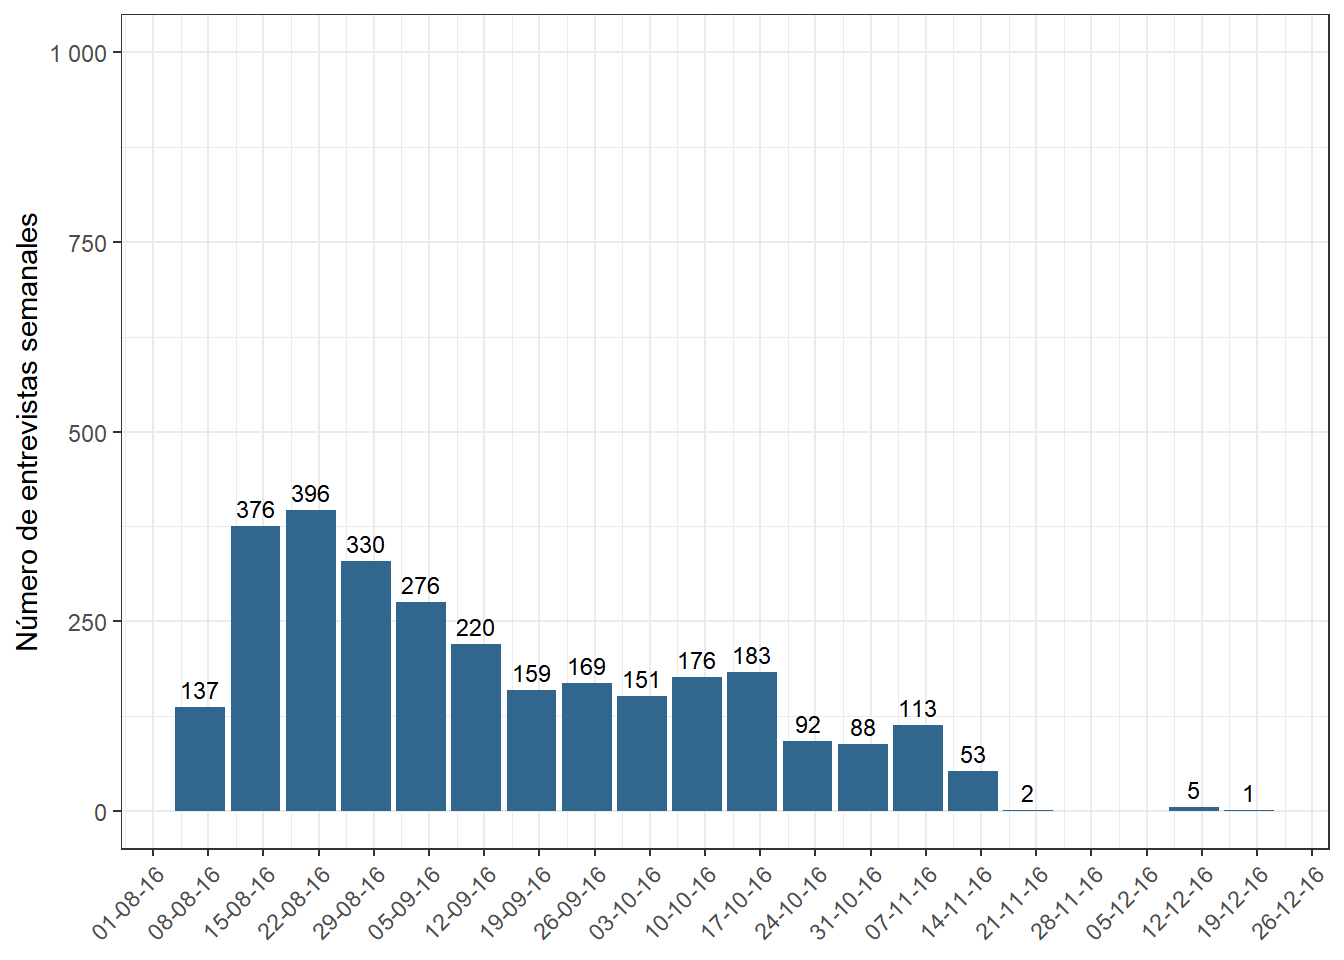
\includegraphics{manual-metodologico-elsoc_files/figure-latex/graf-fechas-ola1-1} 

}

\caption{Número de entrevistas por semana, ola 2016}\label{fig:graf-fechas-ola1}
\end{figure}

\hypertarget{indicadores-levantamiento}{%
\paragraph*{Indicadores levantamiento}\label{indicadores-levantamiento}}
\addcontentsline{toc}{paragraph}{Indicadores levantamiento}

A continuación se presentan las Tasas de Respuesta 1 (TRR1, definida por la AAPOR), Tasa de Cooperación 1 (TCC1), Tasa de Rechazo 1 (TR1) y Tasa de Contacto 1 (TC1)\footnote{Para mayor información sobre la determinación de los códigos de disposición final de casos y el cálculo de las tasas de resultados, ver
  \href{http://www.aapor.org/AAPOR_Main/media/publications/Standard-Definitions20169theditionfinal.pdf}{AAPOR (2016). Standard Definitions. Final Dispositions of Case Codes and Outcome Rates for Surveys}}

\begin{table}[H]

\caption{\label{tab:tabla-tasas-ola1}Tasas de Respuesta, Cooperación, de Rechazo y de Contacto, ola 2016}
\centering
\begin{tabular}[t]{lc}
\toprule
Indicador & Muestra Original\\
\midrule
Tasa de contacto & 72.6\%\\
Tasa de cooperación & 86.0\%\\
Tasa de rechazo & 8.9\%\\
Tasa de respuesta & 62.4\%\\
\bottomrule
\end{tabular}
\end{table}

\hypertarget{casos-falsificados}{%
\paragraph*{Corrección de datos por casos anómalos: Olas 2016 y 2017}\label{casos-falsificados}}
\addcontentsline{toc}{paragraph}{Corrección de datos por casos anómalos: Olas 2016 y 2017}

En el contexto de la ejecución de la tercera ola del estudio ELSOC (año 2018) se diagnosticó la falsificación de un número acotado de casos a lo largo del estudio en las olas 2016 y 2017.

Durante la etapa de supervisión del trabajo de encuestadores durante el 2018, tercera ola de ELSOC, el Centro de Microdatos (CMD) detectó e informó que un conjunto de casos incluidos en la muestra panel son falsos.

Debido al lento avance de las metas de campo de ELSOC en 2018 en Tarapacá y Valparaíso, se enviaron nuevos encuestadores, los cuales detectaron estos problemas. En específico, las encuestas fueron sistemáticamente falsificadas: se realizaron a otras personas no incluídas en la muestra, o los encuestadores solicitaron información a terceros.

Esto llevó a un proceso exhaustivo de revisión, en la cual se detectaron 56 casos falsificados en el campo de 2016 y 47 en el campo de 2017, concentrados en las regiones de Tarapacá (11 casos en 2016 y 11 en 2017) y Valparaíso (45 casos en 2016 y 37 en 2017).

La estrategia de campo de CMD se centra en encuestadores experimentados, asignando los mismos casos a los encuestadores en el tiempo, acorde a la recomendación de la literatura especializada. El problema se concentró en algunos encuestadores específicos en dichas zonas, el cual no fue detectado durante la supervisión de campo de las dos primeras olas.

Los casos falsificados representan el 1,9\% del tamaño muestral efectivo de ELSOC 2016 (N = 2.984) y 1,9\% de 2017 (N = 2.522), por lo que se considera que éstos tienen un impacto marginal a nivel general. A pesar de esto, se tomó la decisión de excluir de las bases de datos los casos falsificados, y se generó y puso a disposición una versión corregida de las bases de datos 2016 y 2017. Los ponderadores fueron corregidos considerando la eliminación de estos casos.

Para evitar estos problemas en el futuro, se modificaron los protocolos de supervisión, aumentando la supervisión presencial y el porcentaje de casos supervisados por encuestador. Adicionalmente, se implementó un sistema de rotación de encuestadores de tal manera que la muestra no sea levantada por los mismos encuestadores en más de una ronda.

\hypertarget{implementaciuxf3n-ola-2017}{%
\subsubsection{Implementación Ola 2017}\label{implementaciuxf3n-ola-2017}}

El levantamiento definitivo de la encuesta se llevó a cabo en un período de doce semanas, durante los meses de julio y octubre de 2017 (ver Figura \ref{fig:graf-fechas-ola2}). Para la ejecución del terreno se contó con 120 encuestadores distribuidos en las 17 sedes de trabajo.

El terreno se llevó a cabo en un período mayor al pronosticado, pues se estimó que duraría nueve semanas, extendiéndose finalmente a doce. Sin embargo, el levantamiento de datos tuvo una duración menor al de la primera ola, que se extendió por 20 semanas. Esta mayor rapidez fue propiciada por la disponibilidad de datos de contacto de los encuestados obtenido en la ola anterior.

La extensión del terreno por sobre la estimación original se debió principalmente a que en las regiones Metropolitana y de Valparaíso existió una mayor dificultad para contactar a los encuestados.

El cierre definitivo del trabajo de campo del levantamiento de la encuesta se desarrolló una vez cubierta la totalidad de la muestra. El terreno se cerró finalmente con 2.521 encuestas realizadas.

\begin{figure}

{\centering 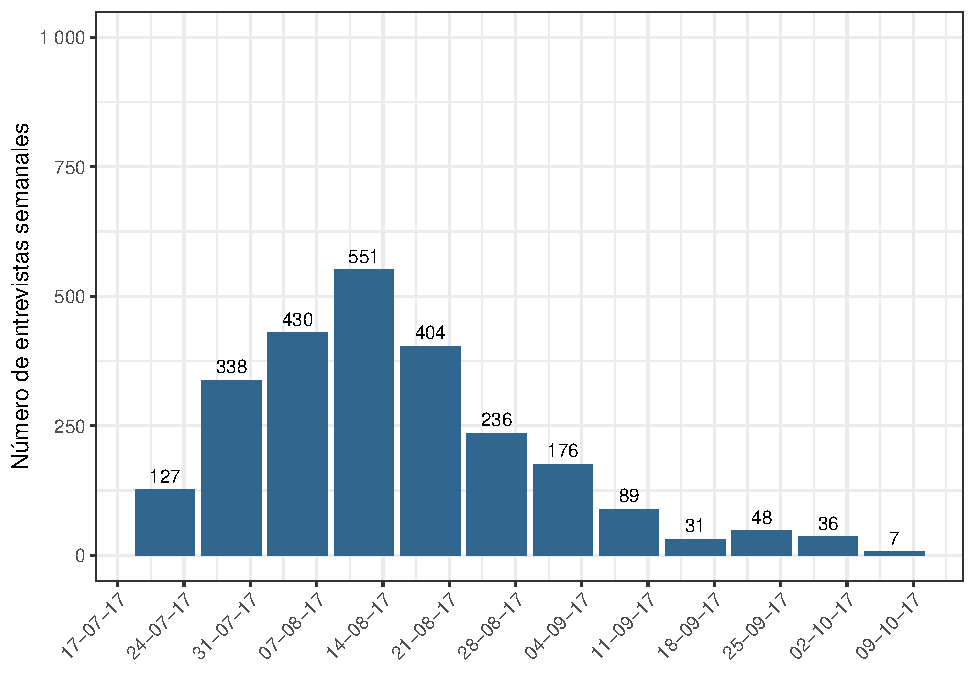
\includegraphics{manual-metodologico-elsoc_files/figure-latex/graf-fechas-ola2-1} 

}

\caption{Número de entrevistas por semana, ola 2017}\label{fig:graf-fechas-ola2}
\end{figure}

\hypertarget{indicadores-levantamiento-1}{%
\paragraph*{Indicadores levantamiento}\label{indicadores-levantamiento-1}}
\addcontentsline{toc}{paragraph}{Indicadores levantamiento}

A continuación se presentan las Tasas de Respuesta 1 (TRR1, definida por la AAPOR), Tasa de Cooperación 1 (TCC1), Tasa de Rechazo 1 (TR1) y Tasa de Contacto 1 (TC1):

\begin{table}[H]

\caption{\label{tab:tabla-tasas-ola2}Tasas de Respuesta, Cooperación, de Rechazo y de Contacto, ola 2017}
\centering
\begin{tabular}[t]{lc}
\toprule
Indicador & Muestra Original\\
\midrule
Tasa de contacto & 88.7\%\\
Tasa de cooperación & 93.1\%\\
Tasa de rechazo & 6.0\%\\
Tasa de respuesta & 82.6\%\\
\bottomrule
\end{tabular}
\end{table}

\hypertarget{casos-falsificados-en-ola-2017}{%
\paragraph{Casos falsificados en ola 2017}\label{casos-falsificados-en-ola-2017}}

Luego de los registros y procedimientos aplicados por el CMD el año 2018 se encontraron y corrigieron anomalías en encuestas realizadas en 2016 y 2017. Para más detalle del problema encontrado y su corrección revisar \protect\hyperlink{casos-falsificados}{Corrección de datos por casos falsificados: Olas 2016 y 2017}.

\hypertarget{implementaciuxf3n-ola-2018}{%
\subsubsection{Implementación Ola 2018}\label{implementaciuxf3n-ola-2018}}

El trabajo de terreno se desarrolló durante los meses de agosto a diciembre de 2018, dentro del tiempo estimado (15 semanas, aproximadamente) (ver Figura \ref{fig:graf-fechas-ola3}). Para la ejecución del terreno se contó con 189 encuestadores distribuidos en 18 sedes de trabajo.

Durante este levantamiento se incluyó la muestra de Refresco, lo que generó una dificultad para los encuestadores, ya que éstos deben explicar y motivar la participación en el estudio, tanto al grupo familiar como a los propios entrevistados.

Por otra parte, la muestra de seguimiento (muestra Original) de los entrevistados 2016-2017 tuvo dificultades de contactabilidad, debido a una mayor presencia de cambios de domicilios registrados que en las versiones anteriores de la encuesta. El 6,9\% se había cambiado a un domicilio diferente.

Otra de las dificultades enfrentadas en ola tiene relación con los casos de falsificación detectados (ver \protect\hyperlink{casos-falsificados}{Corrección de datos por casos falsificados: Olas 2016 y 2017}). Este problema implicó una revisión exhaustiva en terreno de estos casos, y un fortalecimiento al sistema de control, contemplando lo siguiente:

\begin{enumerate}
\def\labelenumi{\arabic{enumi}.}
\item
  Aumentar el porcentaje de encuestas a controlar, de 10\% a un 15\% el 2018. Asegurando controlar al menos el 20\% del trabajo realizado por cada encuestador.
\item
  Estipular para futuras olas del proyecto rotación de los encuestadores sobre el mismo entrevistado.
\item
  Registro de las encuestadoras involucradas de manera de no ser consideradas en futuras
  aplicaciones del estudio. Respecto a la dinámica general del trabajo, se crearon incentivos económicos para que los encuestadores lograran la muestra esperada. Así mismo, se dispuso la movilización necesaria para que los encuestadores cubrieran toda la muestra en los distintos horarios.
\end{enumerate}

El cierre definitivo del trabajo de campo del levantamiento de la encuesta se desarrolló de común acuerdo con COES, una vez cubierta la totalidad de la muestra. El terreno se cerró con 2.274 encuestas en la muestra de seguimiento y 1.523 encuestas en la muestra de refresco.

\begin{figure}

{\centering 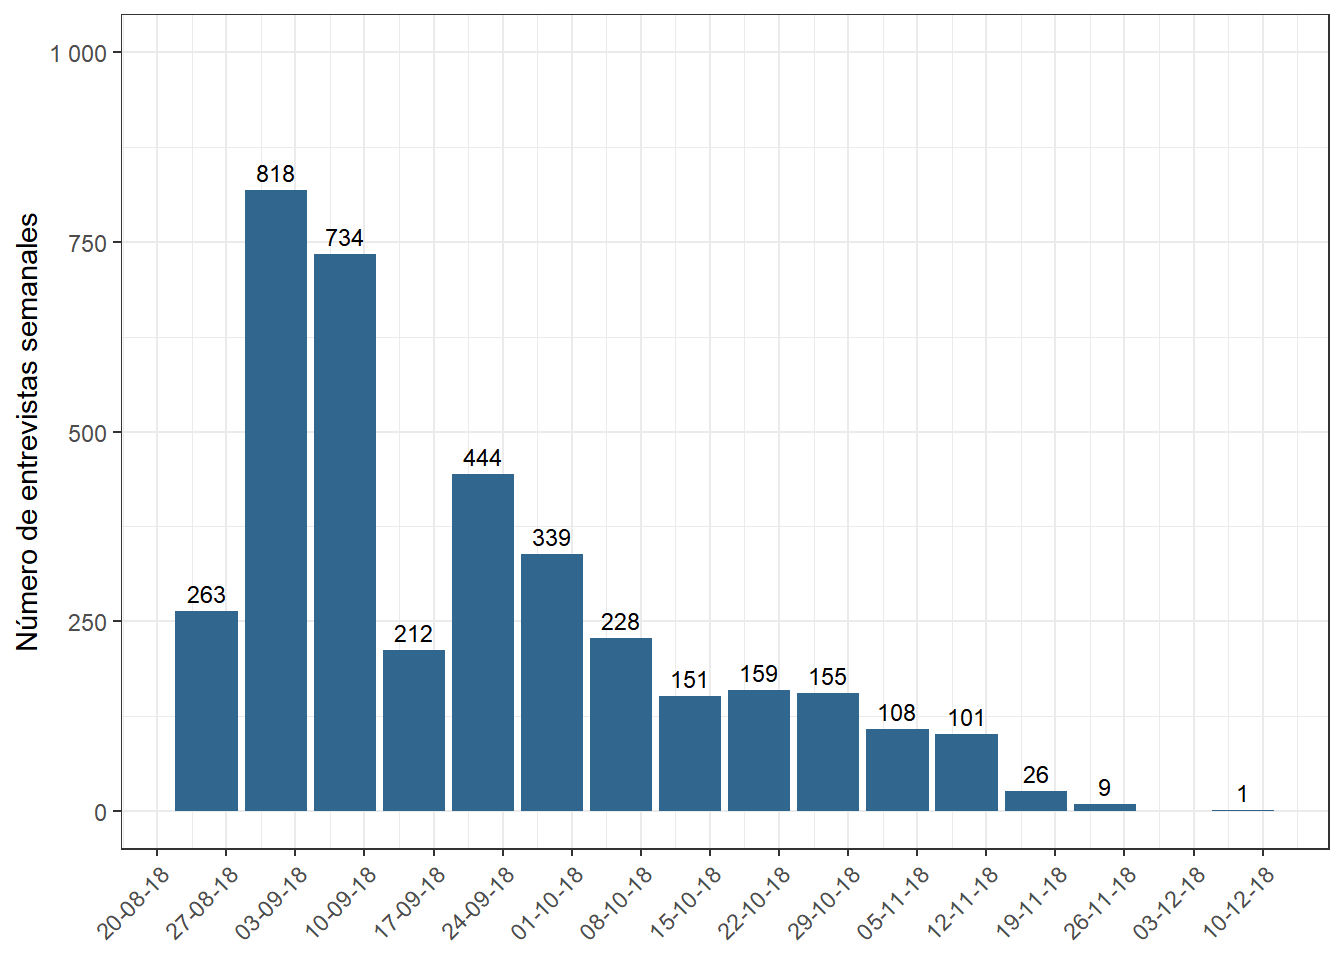
\includegraphics{manual-metodologico-elsoc_files/figure-latex/graf-fechas-ola3-1} 

}

\caption{Número de entrevistas por semana, ola 2018}\label{fig:graf-fechas-ola3}
\end{figure}

\hypertarget{indicadores-levantamiento-2}{%
\paragraph*{Indicadores levantamiento}\label{indicadores-levantamiento-2}}
\addcontentsline{toc}{paragraph}{Indicadores levantamiento}

A continuación se presentan las Tasas de Respuesta 1 (TRR1, definida por la AAPOR), Tasa de Cooperación 1 (TCC1), Tasa de Rechazo 1 (TR1) y Tasa de Contacto 1 (TC1):

\begin{table}[H]

\caption{\label{tab:tabla-tasas-ola3}Tasas de Respuesta, Cooperación, de Rechazo y de Contacto, ola 2018}
\centering
\begin{tabular}[t]{lcc}
\toprule
Indicador & Muestra Original & Muestra Refresco\\
\midrule
Tasa de contacto & 86.0\% & 66.0\%\\
Tasa de cooperación & 93.0\% & 88.0\%\\
Tasa de rechazo & 5.0\% & 8.0\%\\
Tasa de respuesta & 80.0\% & 58.0\%\\
\bottomrule
\end{tabular}
\end{table}

\hypertarget{implementaciuxf3n-ola-2019}{%
\subsubsection{Implementación Ola 2019}\label{implementaciuxf3n-ola-2019}}

El levantamiento de datos de ELSOC 2019 estaba programado para comenzar el sábado 19 de octubre de 2019, sin embargo debido al Estallido Social ocurrido en Chile a partir del 18 de octubre de 2019, el trabajo de terreno debió ser suspendido hasta el jueves 21 de noviembre, fecha en que se inició finalmente la recolección de la información. Por lo tanto, el levantamiento se realizó durante el período de Estallido Social, lo que dificultó su ejecución.

Esta labor se extendió por un periodo de 13 semanas (Dado el desgaste propio de la muestra y del equipo de terreno, se decidió hacer una pausa en el levantamiento de datos durante las últimas 3 semanas de febrero de 2020) (ver Figura \ref{fig:graf-fechas-ola4}). Para la ejecución del terreno se contó con 143 encuestadores distribuidos en 16 sedes de trabajo, administradas por coordinadores de zona debidamente capacitados.

\begin{figure}

{\centering 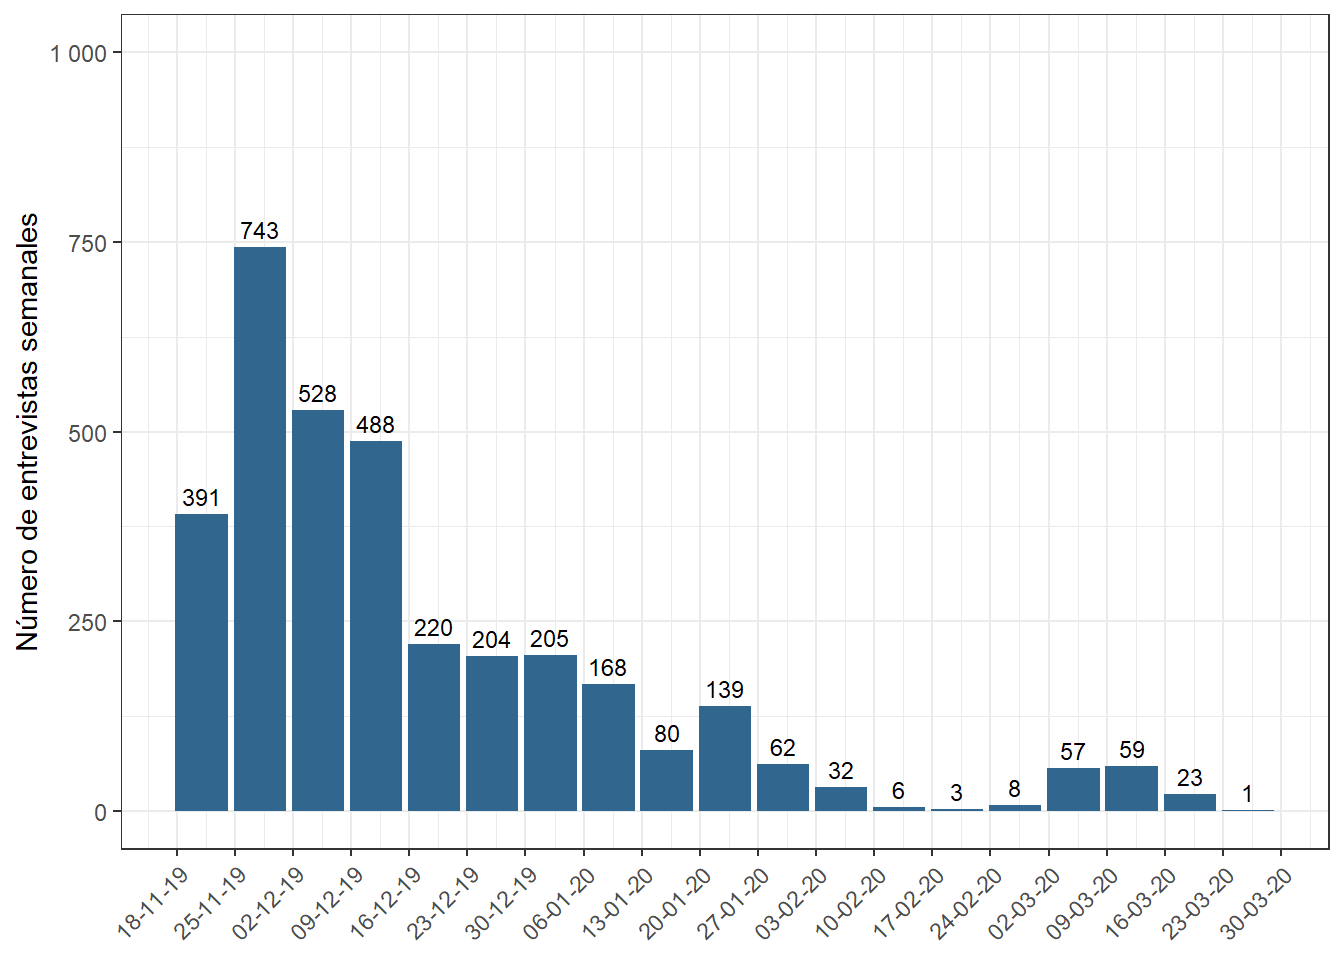
\includegraphics{manual-metodologico-elsoc_files/figure-latex/graf-fechas-ola4-1} 

}

\caption{Número de entrevistas por semana, ola 2019}\label{fig:graf-fechas-ola4}
\end{figure}

\hypertarget{indicadores-levantamiento-3}{%
\paragraph*{Indicadores levantamiento}\label{indicadores-levantamiento-3}}
\addcontentsline{toc}{paragraph}{Indicadores levantamiento}

A continuación se presentan las Tasas de Respuesta 1 (TRR1, definida por la AAPOR), Tasa de Cooperación 1 (TCC1), Tasa de Rechazo 1 (TR1) y Tasa de Contacto 1 (TC1):

\begin{table}[H]

\caption{\label{tab:tabla-tasas-ola4}Tasas de Respuesta, Cooperación, de Rechazo y de Contacto, ola 2019}
\centering
\begin{tabular}[t]{lcc}
\toprule
Indicador & Muestra Original & Muestra Refresco\\
\midrule
Tasa de contacto & 86.0\% & 87.0\%\\
Tasa de cooperación & 93.0\% & 95.0\%\\
Tasa de rechazo & 5.0\% & 3.0\%\\
Tasa de respuesta & 80.0\% & 83.0\%\\
\bottomrule
\end{tabular}
\end{table}

\hypertarget{implementaciuxf3n-ola-2021}{%
\subsubsection{Implementación Ola 2021}\label{implementaciuxf3n-ola-2021}}

La crisis sanitaria producida por la pandemia de COVID-19 y las restricciones asociadas, implicaron cambiar la metodología de aplicación de la Encuesta Longitudinal Social de Chile de forma presencial a remota a través de una encuesta telefónica (Para más detalle ver \protect\hyperlink{instrumento-covid}{Cuestionario 2021: levantamiento durante la pandemia de COVID-19}). Este cambio en la forma de levantar los datos, presentó un gran desafío logístico y operativo, ya que desde sus orígenes ELSOC se había levantado de manera presencial.

La pandemia de COVID-19 también afectó la fecha tradicional de levantamiento de ELSOC, la cual estaba programada para comenzar durante octubre de 2020, sin embargo, el levantamiento de la quinta ola se inició el sábado 30 de enero de 2021 con la asignación de la muestra a los encuestadores capacitados. Las razones para postergar el período de levantamiento fueron principalmente por la espera de condiciones sanitarias y de cuarentenas más favorables que permitieran un levantamiento presencial (sin embargo, prontamente se volvió clara la imposibilidad de mantener la modalidad presencial); y por el tiempo adicional que tomó la preparación del terreno, producto del cambio de modalidad de levantamiento. El trabajo de campo se extendió hasta mediados de junio de 2021. Sin embargo, la aplicación se realizó mayoritariamente entre febrero y abril de 2021 (ver Figura \ref{fig:graf-fechas-ola5}).

Debido al degaste de la muestra y al desgaste del equipo de encuestadores por intentos infructuosos de contacto, es que a contar del mes de mayo se decidió cambiar la metodología de aplicación de producción por unidad muestral a conformar un grupo de encuestadores dedicado exclusivamente a repasar la muestra en una jornada laboral determinada.

\begin{figure}

{\centering 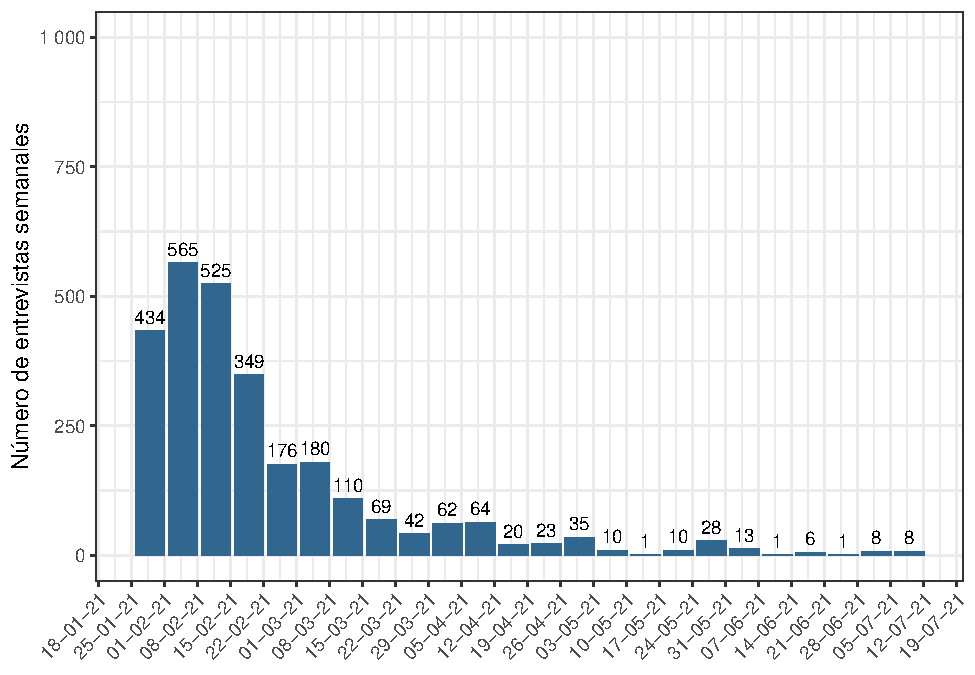
\includegraphics{manual-metodologico-elsoc_files/figure-latex/graf-fechas-ola5-1} 

}

\caption{Número de entrevistas por semana, ola 2021}\label{fig:graf-fechas-ola5}
\end{figure}

\hypertarget{indicadores-levantamiento-4}{%
\paragraph*{Indicadores levantamiento}\label{indicadores-levantamiento-4}}
\addcontentsline{toc}{paragraph}{Indicadores levantamiento}

A continuación se presentan las Tasas de Respuesta 1 (TRR1, definida por la AAPOR), Tasa de Cooperación 1 (TCC1), Tasa de Rechazo 1 (TR1) y Tasa de Contacto 1 (TC1):

\begin{table}[H]

\caption{\label{tab:tabla-tasas-ola5}Tasas de Respuesta, Cooperación, de Rechazo y de Contacto, ola 2021}
\centering
\begin{tabular}[t]{lcc}
\toprule
Indicador & Muestra Original & Muestra Refresco\\
\midrule
Tasa de contacto & 78.0\% & 87.3\%\\
Tasa de cooperación & 83.7\% & 76.1\%\\
Tasa de rechazo & 11.0\% & 8.8\%\\
Tasa de respuesta & 65.2\% & 66.5\%\\
\bottomrule
\end{tabular}
\end{table}

\hypertarget{implementaciuxf3n-ola-2022}{%
\subsubsection{Implementación Ola 2022}\label{implementaciuxf3n-ola-2022}}

El proceso de levantamiento de datos se inició el viernes 22 de julio del 2022, con la asignación de la muestra a los encuestadores capacitados y seleccionados para el estudio, luego de haber realizado el proceso de reclutamiento y selección a nivel nacional. Esta labor se extendió por un periodo de 19 semanas, para culminar el 1 de diciembre de 2022 (ver Figura \ref{fig:graf-fechas-ola6}).

Como resultado, el Plebiscito Constitucional de Salida 2022 ocurrió durante el proceso de levantamiento (realizado el domingo 4 de septiembre), lo que obligó a actualizar las preguntas del cuestionario relacionadas a dicho plebiscito. En particular, se modificó la pregunta acerca del plebiscito, eliminando la que hacía referencia a su intención de voto y añadiendo, en cambio, dos preguntas nuevas: la primera hace referencia a si la persona participó o no en la votación del plebiscito, y la segunda al voto retrospectivo en cuestión.

\begin{figure}

{\centering 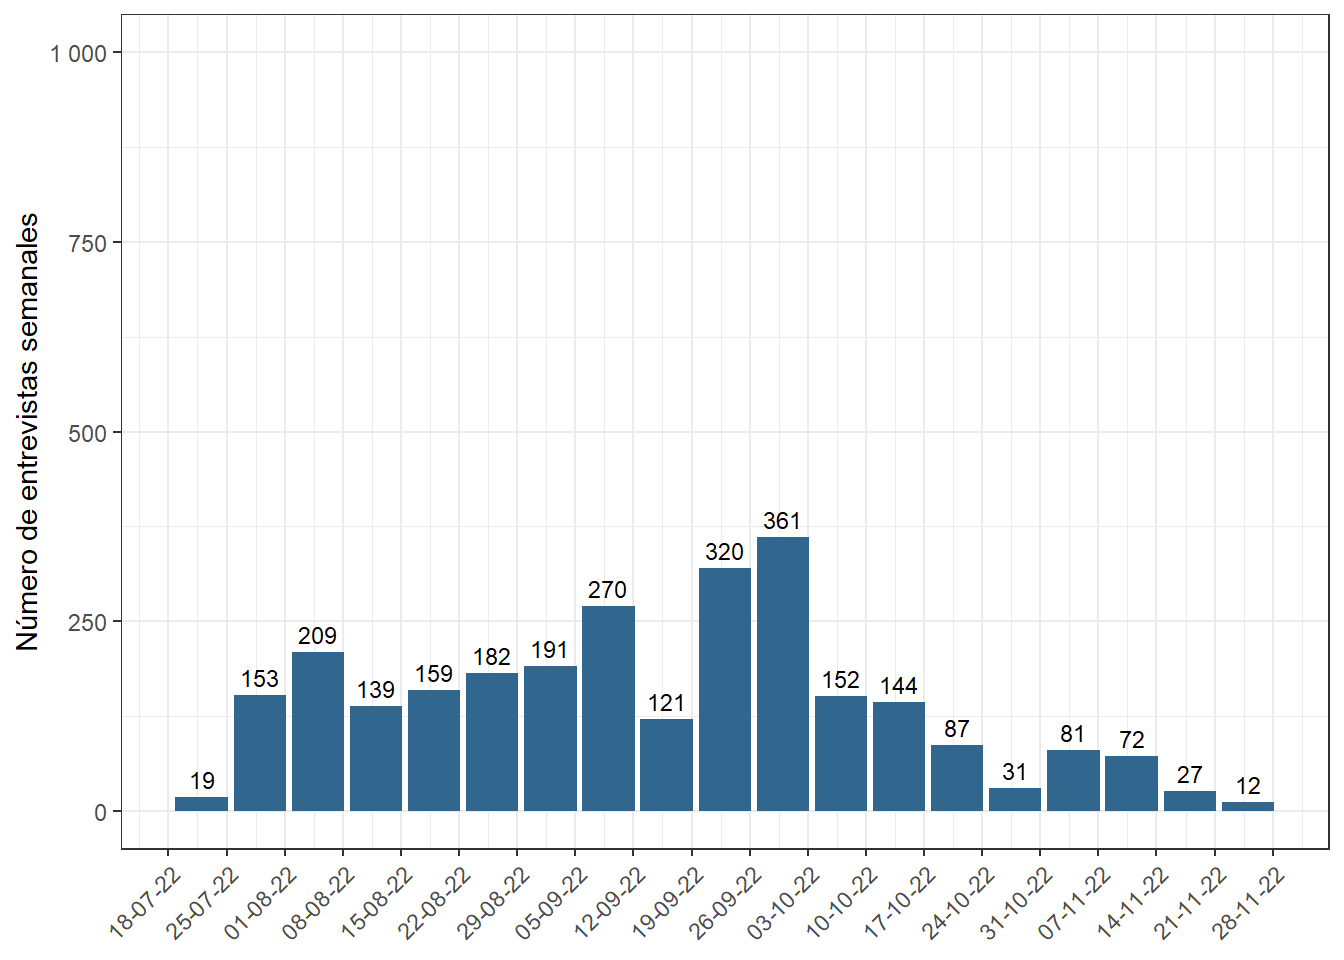
\includegraphics{manual-metodologico-elsoc_files/figure-latex/graf-fechas-ola6-1} 

}

\caption{Número de entrevistas por semana, ola 2022}\label{fig:graf-fechas-ola6}
\end{figure}

\hypertarget{indicadores-levantamiento-5}{%
\paragraph*{Indicadores levantamiento}\label{indicadores-levantamiento-5}}
\addcontentsline{toc}{paragraph}{Indicadores levantamiento}

A continuación se presentan las Tasas de Respuesta 1 (TRR1, definida por la AAPOR), Tasa de Cooperación 1 (TCC1), Tasa de Rechazo 1 (TR1) y Tasa de Contacto 1 (TC1):

\begin{table}[H]

\caption{\label{tab:tabla-tasas-ola6}Tasas de Respuesta, Cooperación, de Rechazo y de Contacto, ola 2022}
\centering
\begin{tabular}[t]{lcc}
\toprule
Indicador & Muestra Original & Muestra Refresco\\
\midrule
Tasa de contacto & 79.1\% & 79.1\%\\
Tasa de cooperación & 83.0\% & 84.8\%\\
Tasa de rechazo & 12.1\% & 10.9\%\\
Tasa de respuesta & 65.6\% & 67.1\%\\
\bottomrule
\end{tabular}
\end{table}

\hypertarget{indicadores-levantamiento-6}{%
\subsection{Indicadores levantamiento}\label{indicadores-levantamiento-6}}

A continuación, se muestran las tasas de contacto, cooperación, rechazo y respuesta para todas las muestras y olas.

\begin{table}[H]

\caption{\label{tab:tabla-de-tasas-varias-olas}Tasas de Respuesta, de Cooperación, de Rechazo y de Contacto, según ola y muestra}
\centering
\begin{tabular}[t]{ccccc}
\toprule
Ola & Tasa de Respuesta & Tasa de Cooperación & Tasa de Rechazo & Tasa de Contacto\\
\midrule
\addlinespace[0.3em]
\multicolumn{5}{l}{\textbf{Muestra Original}}\\
\hspace{1em}2016 & 62.4\% & 86.0\% & 8.9\% & 72.6\%\\
\hspace{1em}2017 & 82.6\% & 93.1\% & 6.0\% & 88.7\%\\
\hspace{1em}2018 & 80.0\% & 93.0\% & 5.0\% & 86.0\%\\
\hspace{1em}2019 & 80.0\% & 93.0\% & 5.0\% & 86.0\%\\
\hspace{1em}2021 & 65.2\% & 83.7\% & 11.0\% & 78.0\%\\
\hspace{1em}2022 & 65.6\% & 83.0\% & 12.1\% & 79.1\%\\
\addlinespace[0.3em]
\multicolumn{5}{l}{\textbf{Muestra Refresco}}\\
\hspace{1em}2018 & 58.0\% & 88.0\% & 8.0\% & 66.0\%\\
\hspace{1em}2019 & 83.0\% & 95.0\% & 3.0\% & 87.0\%\\
\hspace{1em}2021 & 66.5\% & 76.1\% & 8.8\% & 87.3\%\\
\hspace{1em}2022 & 67.1\% & 84.8\% & 10.9\% & 79.1\%\\
\bottomrule
\end{tabular}
\end{table}

\hypertarget{atricion}{%
\subsection{Atrición de la encuesta}\label{atricion}}

A continuación, se presenta la atrición obtenida según Muestra:

\begin{table}[H]

\caption{\label{tab:tabla-atricion}Atrición de las muestras de ELSOC entre olas}
\centering
\begin{tabular}[t]{ccccc}
\toprule
\multicolumn{1}{c}{ } & \multicolumn{2}{c}{Muestra Lograda} & \multicolumn{2}{c}{Tasa de Atrición} \\
\cmidrule(l{3pt}r{3pt}){2-3} \cmidrule(l{3pt}r{3pt}){4-5}
Medición & Muestra Original & Muestra Refresco & Muestra Original & Muestra Refresco\\
\midrule
2016 & 2927 &  &  & \\
2017 & 2473 &  & 15.5\% & \\
2018 & 2229 & 1519 & 9.9\% & \\
2019 & 2153 & 1264 & 3.4\% & 16.8\%\\
2021 & 1739 & 1001 & 19.2\% & 20.8\%\\
\addlinespace
2022 & 1728 & 1002 & 0.6\% & -0.1\%\\
\bottomrule
\end{tabular}
\end{table}

\begin{itemize}
\tightlist
\item
  Según sexo:
\end{itemize}

\begin{table}[H]

\caption{\label{tab:tabla-atricion-sexo}Atrición de las muestras de ELSOC entre olas, según sexo}
\centering
\begin{tabular}[t]{ccccc}
\toprule
\multicolumn{1}{c}{ } & \multicolumn{2}{c}{Muestra Lograda} & \multicolumn{2}{c}{Tasa de Atrición} \\
\cmidrule(l{3pt}r{3pt}){2-3} \cmidrule(l{3pt}r{3pt}){4-5}
Medición & Hombres & Mujeres & Hombres & Mujeres\\
\midrule
\addlinespace[0.3em]
\multicolumn{5}{l}{\textbf{Muestra Original}}\\
\hspace{1em}2016 & 1163 & 1764 &  & \\
\hspace{1em}2017 & 953 & 1520 & 18.1\% & 13.8\%\\
\hspace{1em}2018 & 841 & 1387 & 11.8\% & 8.8\%\\
\hspace{1em}2019 & 807 & 1346 & 4.0\% & 3.0\%\\
\hspace{1em}2021 & 631 & 1108 & 21.8\% & 17.7\%\\
\hspace{1em}2022 & 615 & 1113 & 2.5\% & -0.5\%\\
\addlinespace[0.3em]
\multicolumn{5}{l}{\textbf{Muestra Refresco}}\\
\hspace{1em}2018 & 607 & 912 &  & \\
\hspace{1em}2019 & 482 & 782 & 20.6\% & 14.3\%\\
\hspace{1em}2021 & 378 & 623 & 21.6\% & 20.3\%\\
\hspace{1em}2022 & 377 & 625 & 0.3\% & -0.3\%\\
\bottomrule
\end{tabular}
\end{table}

\begin{itemize}
\tightlist
\item
  Según tramo etareo:
\end{itemize}

\begin{table}[H]

\caption{\label{tab:tabla-atricion-edad}Atrición de las muestras de ELSOC entre olas, según tramo etáreo}
\centering
\begin{tabular}[t]{ccccccccc}
\toprule
\multicolumn{1}{c}{ } & \multicolumn{4}{c}{Muestra Lograda} & \multicolumn{4}{c}{Tasa de Atrición} \\
\cmidrule(l{3pt}r{3pt}){2-5} \cmidrule(l{3pt}r{3pt}){6-9}
Medición & 19-29 & 30-49 & 50-64 & 65 o más & 19-29 & 30-49 & 50-64 & 65 o más\\
\midrule
\addlinespace[0.3em]
\multicolumn{9}{l}{\textbf{Muestra Original}}\\
\hspace{1em}2016 & 506 & 1157 & 839 & 425 &  &  &  & \\
\hspace{1em}2017 & 407 & 962 & 734 & 370 & 19.6\% & 16.9\% & 12.5\% & 12.9\%\\
\hspace{1em}2018 & 340 & 863 & 687 & 338 & 16.5\% & 10.3\% & 6.4\% & 8.6\%\\
\hspace{1em}2019 & 327 & 838 & 666 & 322 & 3.8\% & 2.9\% & 3.1\% & 4.7\%\\
\hspace{1em}2021 & 269 & 685 & 546 & 239 & 17.7\% & 18.3\% & 18.0\% & 25.8\%\\
\hspace{1em}2022 & 276 & 648 & 565 & 239 & -2.6\% & 5.4\% & -3.5\% & 0.0\%\\
\addlinespace[0.3em]
\multicolumn{9}{l}{\textbf{Muestra Refresco}}\\
\hspace{1em}2018 & 341 & 579 & 418 & 181 &  &  &  & \\
\hspace{1em}2019 & 271 & 472 & 369 & 152 & 20.5\% & 18.5\% & 11.7\% & 16.0\%\\
\hspace{1em}2021 & 216 & 391 & 282 & 112 & 20.3\% & 17.2\% & 23.6\% & 26.3\%\\
\hspace{1em}2022 & 209 & 382 & 294 & 117 & 3.2\% & 2.3\% & -4.3\% & -4.5\%\\
\bottomrule
\end{tabular}
\end{table}

\begin{itemize}
\tightlist
\item
  Según nivel educacional:
\end{itemize}

\begin{table}[H]

\caption{\label{tab:tabla-atricion-educ}Atrición de las muestras de ELSOC entre olas, según nivel educacional}
\centering
\begin{tabular}[t]{ccccccccc}
\toprule
\multicolumn{1}{c}{ } & \multicolumn{4}{c}{Muestra Lograda} & \multicolumn{4}{c}{Tasa de Atrición} \\
\cmidrule(l{3pt}r{3pt}){2-5} \cmidrule(l{3pt}r{3pt}){6-9}
Medición & Básica & Media & Técnica & Univ & Básica & Media & Técnica & Univ\\
\midrule
\addlinespace[0.3em]
\multicolumn{9}{l}{\textbf{Muestra Original}}\\
\hspace{1em}2016 & 656 & 1251 & 483 & 535 &  &  &  & \\
\hspace{1em}2017 & 580 & 1062 & 396 & 434 & 11.6\% & 15.1\% & 18.0\% & 18.9\%\\
\hspace{1em}2018 & 512 & 977 & 358 & 380 & 11.7\% & 8.0\% & 9.6\% & 12.4\%\\
\hspace{1em}2019 & 490 & 953 & 341 & 368 & 4.3\% & 2.5\% & 4.7\% & 3.2\%\\
\hspace{1em}2021 & 363 & 757 & 283 & 336 & 25.9\% & 20.6\% & 17.0\% & 8.7\%\\
\hspace{1em}2022 & 402 & 752 & 265 & 308 & -10.7\% & 0.7\% & 6.4\% & 8.3\%\\
\addlinespace[0.3em]
\multicolumn{9}{l}{\textbf{Muestra Refresco}}\\
\hspace{1em}2018 & 283 & 633 & 253 & 347 &  &  &  & \\
\hspace{1em}2019 & 254 & 537 & 206 & 264 & 10.2\% & 15.2\% & 18.6\% & 23.9\%\\
\hspace{1em}2021 & 167 & 426 & 175 & 233 & 34.3\% & 20.7\% & 15.0\% & 11.7\%\\
\hspace{1em}2022 & 197 & 424 & 163 & 218 & -18.0\% & 0.5\% & 6.9\% & 6.4\%\\
\bottomrule
\end{tabular}
\end{table}

\hypertarget{atriciuxf3n-respecto-a-otras-encuestas}{%
\subsubsection{Atrición respecto a otras encuestas}\label{atriciuxf3n-respecto-a-otras-encuestas}}

A continuación, se presenta la muestra alcanzada por encuestas longitudinales para investigación social similares a ELSOC, realizadas en otras partes del mundo. Para el caso de The UK Household Longitudinal Study, de Understanding Society, se encuentran las siguientes muestras alcanzadas y tasas de atrición por medición:

\begin{table}[H]
\centering
\begin{tabular}[t]{lcccccccc}
\toprule
\multicolumn{1}{c}{ } & \multicolumn{4}{c}{Muestra Lograda} & \multicolumn{4}{c}{Tasa de Atrición} \\
\cmidrule(l{3pt}r{3pt}){2-5} \cmidrule(l{3pt}r{3pt}){6-9}
Medición & General 
 Population 
 Sample & British 
 Household 
 Panel 
 Survey & Immigrant and 
 Ethnic Minority 
 Boost Sample & Ethnic Minority Boost Sample & General 
 Population 
 Sample & British 
 Household 
 Panel 
 Survey & Immigrant and 
 Ethnic Minority 
 Boost Sample & Ethnic Minority Boost Sample\\
\midrule
1 & 43674 & - & - & 7320 &  &  &  & \\
2 & 36960 & 11706 & - & 5593 & 15.4\% &  &  & 23.6\%\\
3 & 33248 & 11028 & - & 5099 & 10.0\% & 5.8\% &  & 8.8\%\\
4 & 31674 & 10556 & - & 4902 & 4.7\% & 4.3\% &  & 3.9\%\\
5 & 30103 & 10069 & - & 4709 & 5.0\% & 4.6\% &  & 3.9\%\\
\addlinespace
6 & 27120 & 9429 & 4654 & 4140 & 9.9\% & 6.4\% &  & 12.1\%\\
7 & 25607 & 9050 & 3475 & 3793 & 5.6\% & 4.0\% & 25.3\% & 8.4\%\\
8 & 24053 & 8641 & 3018 & 3535 & 6.1\% & 4.5\% & 13.2\% & 6.8\%\\
9 & 22335 & 8157 & 2444 & 3116 & 7.1\% & 5.6\% & 19.0\% & 11.8\%\\
10 & 21479 & 7712 & 2219 & 2908 & 3.8\% & 5.4\% & 9.2\% & 6.7\%\\
\addlinespace
11 & 20011 & 7430 & 1866 & 2699 & 6.8\% & 3.6\% & 15.9\% & 7.2\%\\
\bottomrule
\end{tabular}
\end{table}

Para el caso de The New Zealand Attitudes and Values Study (NZAVS), se encuentra la siguiente muestra alcanzada y atrición por medición:

\begin{table}[H]
\centering
\begin{tabular}[t]{lccccc}
\toprule
\multicolumn{1}{c}{ } & \multicolumn{2}{c}{Muestra Lograda} & \multicolumn{3}{c}{Tasa de Atrición} \\
\cmidrule(l{3pt}r{3pt}){2-3} \cmidrule(l{3pt}r{3pt}){4-6}
Medición & Prov. de 1ra Medición & Prov. de Medición Anterior & M. Total Acumulada & Relativa a 1ra Medición & Relativa a Medición Anterior\\
\midrule
1.0 & - & - & 6518 &  & \\
2.0 & 4425 & 4425 & 4441 & 32.1\% & 32.1\%\\
3.0 & 3918 & 3921 & 6884 & 39.9\% & 11.7\%\\
3.5 & 1977 & 2113 & 4514 & 69.7\% & 69.3\%\\
4.0 & 4053 & 5762 & 12979 & 37.8\% & 16.3\%\\
\addlinespace
5.0 & 3934 & 9844 & 18261 & 39.6\% & 24.2\%\\
6.0 & 3728 & 14878 & 15820 & 42.8\% & 18.5\%\\
7.0 & 3344 & 12550 & 13942 & 48.7\% & 20.7\%\\
8.0 & 3347 & 11933 & 21936 & 48.6\% & 14.4\%\\
9.0 & 2771 & 15784 & 17072 & 57.5\% & 28.0\%\\
\addlinespace
10.0 & 2964 & 14049 & 47951 & 54.5\% & 17.7\%\\
11.0 & 2506 & 34782 & 42864 & 61.6\% & 27.5\%\\
12.0 & 2107 & 33318 & 38551 & 67.7\% & 22.3\%\\
\bottomrule
\end{tabular}
\end{table}

\newpage

\hypertarget{bases-datos}{%
\section{Bases de Datos}\label{bases-datos}}

\hypertarget{descarga-de-bases-de-datos}{%
\subsection{Descarga de Bases de datos}\label{descarga-de-bases-de-datos}}

Las bases de datos ELSOC son puestas a disposición al público general en el momento en que se ha completado su proceso de revisión y validación. Las bases de datos son publicadas y archivadas en el repositorio de \textbf{Harvard Dataverse}, en la \href{https://dataverse.harvard.edu/dataverse/coes_data_repository}{carpeta de datos de COES}. Este repositorio permite un acceso gratuito y seguro a las bases de datos.

ELSOC se pone a disposición como bases de datos transversales según ola: olas 2016, 2017, 2018, 2019 y 2021, en formato de datos de R (.RData), SPSS (.sav), Stata 13 (.dta) y Stata 14 (.dta).

Adicionalmente, a partir de 2019, se publican las bases de datos en formato longitudinal, para facilitar su uso como encuesta panel. A la fecha se encuentran publicadas la base longitudinal de olas 2016-2019 en formato wide, y bases longitudinal de olas 2016-2021 en formato wide y long. Las variables que han presentado cambios en el tiempo se encuentran armonizadas para permitir su uso longitudinal.

Como parte de un proceso continuo de mejora, es posible que las bases de datos publicadas sean actualizadas durante el desarrollo de ELSOC, debido a la corrección de potenciales errores, mejoras en el formato de los datos, actualización de códigos de no respuesta, etc. Dado esto, en el repositorio de Harvard Dataverse se encuentra publicada la última versión disponible, así como todas las versiones anteriores en caso de ser necesarias.

\hypertarget{fichas-tuxe9cnicas}{%
\subsection{Fichas Técnicas}\label{fichas-tuxe9cnicas}}

En este apartado se presenta la Ficha Técnica (Ver Cuadro \ref{tab:ficha}, dónde se sintetizan las principales características del Estudio Longitudinal Social de Chile (ELSOC COES):

\begin{longtable}[t]{>{\raggedright\arraybackslash}p{8em}>{\raggedright\arraybackslash}p{35em}}
\caption{\label{tab:ficha}Ficha Técnica ELSOC COES}\\
\toprule
Características & ELSOC\\
\midrule
\endfirsthead
\caption[]{\label{tab:ficha}Ficha Técnica ELSOC COES \textit{(continued)}}\\
\toprule
Características & ELSOC\\
\midrule
\endhead

\endfoot
\bottomrule
\endlastfoot
Objetivo & Analizar longitudinalmente la evolución del conflicto y cohesión
                              en la sociedad chilena\\
Diseño & Estudio cuantitativo por medio de un cuestionario estructurado\\
Instrumento & Cuestionario compuesto por preguntas cerradas de carácter simple y múltiple junto a algunas preguntas abiertas\\
Unidad de análisis & Individuos\\
Población objetivo & Hombres y mujeres de 18 a 75 años, residentes habituales de viviendas particulares\\
\addlinespace
Marco muestral & Marco de muestreo de manzanas del pre-censo 2011, trabajo elaborado por el Centro de Inteligencia Territorial (CIT) de la Universidad Adolfo Ibáñez\\
Diseño muestral & Probabilístico, estratificado, por conglomerados y multietápico\\
Unidades de muestreo & Primero se eligen ciudades (UPM), luego manzanas (USM), y sub-bloques y viviendas (UTM). La unidad final de selección es la persona\\
Periodicidad & Anual. Muestra de refresco a oartir del 3er año\\
Modo de aplicación & Formato CAPI en vivienda del entrevistado. Formato CATI durante 2021\\
\addlinespace
Informante & Hombre o mujer residente en la vivienda, con edad entre 18 y 75 años.\\
Duración promedio & 51 minutos\\
Representatividad & Aproximadamente el 77\% de la población total del país y 93\% de la
              población urbana con la muestra de Ola 2016\\
Organismo responsable & Centro de Estudios del Conflicto y Cohesión Social (COES)\\
Organismo ejecutor & CentroMicroDatos (CMD) de la Universidad de Chile\\*
\end{longtable}

\hypertarget{protocolo-de-uso-de-base-de-datos}{%
\subsection{Protocolo de Uso de Base de Datos}\label{protocolo-de-uso-de-base-de-datos}}

Cualquier publicación que utilize las bases de datos ELSOC, en cualquiera de sus versiones, debe citar la fuente de las siguientes formas (dependiendo de la base utilizada):

\begin{itemize}
\tightlist
\item
  ELSOC 2016:
\end{itemize}

\textbf{Centro de Estudios de Conflicto y Cohesión Social (2016). Estudio Longitudinal Social de Chile, Primera Ola (ELSOC\_W01\_v1.00). {[}Archivo de datos{]}. Santiago, Chile: Centro de Estudios de Conflicto y Cohesión Social (COES). www.coes.cl}

\begin{itemize}
\tightlist
\item
  ELSOC 2017:
\end{itemize}

\textbf{Centro de Estudios de Conflicto y Cohesión Social (2017). Estudio Longitudinal Social de Chile, Segunda Ola (ELSOC\_W02\_v1.00). {[}Archivo de datos{]}. Santiago, Chile: Centro de Estudios de Conflicto y Cohesión Social (COES). www.coes.cl}

\begin{itemize}
\tightlist
\item
  ELSOC 2018:
\end{itemize}

\textbf{Centro de Estudios de Conflicto y Cohesión Social (2018). Estudio Longitudinal Social de Chile, Tercera Ola (ELSOC\_W03\_v1.00). {[}Archivo de datos{]}. Santiago, Chile: Centro de Estudios de Conflicto y Cohesión Social (COES). www.coes.cl}

\begin{itemize}
\tightlist
\item
  ELSOC 2019:
\end{itemize}

\textbf{Centro de Estudios de Conflicto y Cohesión Social (2019). Estudio Longitudinal Social de Chile, Cuarta Ola (ELSOC\_W04\_v1.00). {[}Archivo de datos{]}. Santiago, Chile: Centro de Estudios de Conflicto y Cohesión Social (COES). www.coes.cl}

\begin{itemize}
\tightlist
\item
  ELSOC 2021:
\end{itemize}

\textbf{Centro de Estudios de Conflicto y Cohesión Social (2021). Estudio Longitudinal Social de Chile, Quinta Ola (ELSOC\_W05\_v1.00). {[}Archivo de datos{]}. Santiago, Chile: Centro de Estudios de Conflicto y Cohesión Social (COES). www.coes.cl}

O en su formato longitudinal:

\textbf{Centro de Estudios de Conflicto y Cohesión Social (2021). Estudio Longitudinal Social de Chile, Versión Panel Combinada 2016-2019 (ELSOC\_Wide\_2016\_2019\_v1.00). {[}Archivo de datos{]}. Santiago, Chile: Centro de Estudios de Conflicto y Cohesión Social (COES). www.coes.cl}

Por último, en caso de que se desee citar el presente Manual de Usuario:

\textbf{Centro de Estudios de Conflicto y Cohesión Social (2021). Manual de Usuario de Estudio Longitudinal Social de Chile. Santiago, Chile: Centro de Estudios de Conflicto y Cohesión Social (COES).}

\newpage

\hypertarget{uxe9tica}{%
\section{Ética}\label{uxe9tica}}

\hypertarget{aprobaciuxf3n-comituxe9-de-uxe9tica}{%
\subsection{Aprobación Comité de Ética}\label{aprobaciuxf3n-comituxe9-de-uxe9tica}}

El Estudio Longitudinal sobre Conflicto y Cohesión Social en Chile (ELSOC) cuenta con aprobación ética en todas sus olas del \href{http://eticayseguridad.uc.cl/comite-etico-cientifico-en-ciencias-sociales-artes-y-humanidades.html}{Comité Ético Científico de Ciencias Sociales, Artes y Humanidades de la Pontifícia Universidad Católica de Chile} con fecha 08 de junio de 2016 e \textbf{ID Protocolo 160129004}.

La aprobación del Comité de Ética fue renovada con fecha 06 de enero de 2021.

\hypertarget{consentimiento-informado}{%
\subsection{Consentimiento informado}\label{consentimiento-informado}}

Los participantes del estudio firmaron un Consentimiento Informado por Escrito en que se detallan los objetivos del estudio, en qué consiste su participación y qué se hará y cómo se resguardará la información y datos entregados.

Los participantes del estudio de la Muestra Original firmaron el Consentimiento Informado el 2016, mientras que los participantes de la Muestra Refresco en 2018. Adicionalmente, debido al cambio de modalidad realizado durante el levantamento de la ola 2021 (ver \protect\hyperlink{instrumento-covid}{Cuestionario 2021: levantamiento durante la pandemia de COVID-19}), se solicitó a los participantes de ambas muestras firmar un Apéndice al Consentimiento Informado, en que se detalló los cambios realizados durante dicha ola.

\newpage

\hypertarget{dudas-y-consultas}{%
\section{Dudas y Consultas}\label{dudas-y-consultas}}

En caso de que detecte problemas con la base de datos, desee plantear solicitudes y/o tenga dudas sobre aspectos no cubiertos por el presente Manual de Usuario, las cuales no puedan ser resueltas por otros medios, puede comunicarse con el Equipo de Encuestas COES al correo electrónico \url{elsoc@uc.cl}. El equipo procesará su solicitud y tratará de contestar en el más breve plazo.

\newpage

\end{document}
